\documentclass[../thesis_main.tex]{subfiles}
\DeclareMathOperator*{\barr}{\scalerel*{+}{\textstyle\sum}}

\begin{document}
\chapter{$\mathbb{Z}_2$ Lattice Gauge Theory}
The principle of gauging symmetries has been one of the most successful paradigms in the history of physics, ranging from the theory of general relativity to the Standard Model of particle physics. Despite the introduction of redundancy, gauging of symmetries is often employed as a guiding principle for constructing physical theories. In condensed matter physics, gauge theories appear as an emergent theory of strongly interacting many-body problems, and gauge description becomes indispensible to understand confined and deconfined phases of matter \cite{Sergej,Mathur_et_al}. 

In this chapter, we will discuss the simplest gauge theory one can define on a lattice $-$ the pure $\mathbb{Z}_2$ lattice gauge theory (without matter fields) with the topology of a torus (periodic boundary conditions), which was discovered by Franz Wegner in 1971 \cite{wegner2014duality}. We will also discuss the Wegner duality which maps the $\mathbb{Z}_2$ gauge theory to the $\mathbb{Z}_2$ Transverse Field Ising model (TFIM) with the \textit{singlet constraint}. To study the phases of this dual theory, we employ the Path Integral Monte Carlo method which further maps the $d$-dimensional TFIM to a $(d+1)$-dimensional generalized classical Ising model which can be simulated using an extended version of the Metropolis algorithm.

\section{Hamiltonian}
The Hamiltonian of $\mathbb{Z}_2$ gauge theory is given by 
\begin{equation}
    \hat{H}_{\mathbb{Z}_2} = - J \sum_{p} \underbrace{\prod_{\ell \: \in \: p} \sigma^z_{\: \ell}}_{\hat{B_p}} \: - h \sum_{\ell} \sigma^x_{\: \ell}
\end{equation}
%%% FIG %%%
\begin{figure}[!htb]
    \centering
    \begin{subfigure}[b]{0.35\textwidth}  %keep total sum <1 to show in same line
        \centering
        \includegraphics[width=\textwidth]{images/z2_gauge_theory/z2_lattice.tex}
    \end{subfigure}
    \caption{ $\mathbb{Z}_2$ gauge theory lattice with degrees of freedom living on the links/edges.}
    \label{z2_lattice}
\end{figure}
%%% FIG %%%
\!\!\!
where the label $\ell$ indexes the links/edges on the lattice and the label $p$ denotes a plaquette (square face) on the lattice. As can be seen from Fig. \ref{z2_lattice}, the $\hat{B_p}$ term looks like a discrete curl and is the $\mathbb{Z}_2$ analog of magnetic flux through the plaquette $p$. Similarly, the $\sigma^x_{\: \ell}$ term is the $\mathbb{Z}_2$ analog of electric flux. This is the simplest Hamiltonian one can construct in terms of gauge invariant $\mathbb{Z}_2$ operators. 
The gauge transformation of a lattice model is given by the local symmetry of the Hamiltonian. For our $\mathbb{Z}_2$ gauge theory Hamiltonian, the gauge transformations are generated by the vertex star operator $\hat{G_v}$.
\begin{equation}
    \hat{G_v} \equiv \prod_{\ell \: \in \: +} \sigma^x_{\: \ell}
\end{equation}
By definition, $\hat{G_v}$ is a local symmetry of the Hamiltonian. 
\begin{equation}
    [\hat{G_v}, \hat{H}] = 0, \quad \forall \: v.
\end{equation}
Therefore, $G_v$ is a conserved quantity. Furthermore, since $G_v$ is a $\mathbb{Z}_2$ operator, it squares to identity.
\begin{equation}
    \hat{G_v}^2 = \mathds{1} \quad \implies \quad G_v = \pm 1, \quad \forall \: v.
\end{equation}    
Different eigenvalues of $G_v$ for a vertex $v$ correspond to different sectors of the Hilbert space. Fixing the value of the eigenvalue $G_v$ acts like a gauge-fixing condition. As noted earlier, the $\sigma^x_{\: \ell}$ term acts like the electric flux analog, i.e., $\sigma^x_{\: \ell} \sim e^{iE_\ell}$. This implies that $\hat{G_v} \sim e^{i \nabla \cdot \vec{E}}$. Therefore, the gauge-fixing condition is also commonly known as the ``Gauss' law constraint''. For the $\mathbb{Z}_2$ Hamiltonian, the Gauss' law constraint can be written as 
\begin{equation}
    G_v \sim e^{i \pi \rho} = \pm 1, \quad \implies \quad \rho \in \{0, 1\} 
\end{equation}
Hence, the $\pm 1$ eigenvalues loosely correspond to the absence or the presence of a $\mathbb{Z}_2$ charge on the vertex $v$, respectively. Since we are interested in probing the low-energy subspace of our problem, we choose the charge-free sector of the Gauss' law constraint
\begin{equation}
    \text{\textbf{Constraint 1:} }G_v = + 1, \quad \forall \: v.
    \label{gausslaw}
\end{equation}
Furthermore, as we are interested in probing the topological properties of this model, we invoke periodic boundary conditions in our system. The periodic boundary conditions naturally lead to another constraint between the operators
\begin{equation}
    \text{\textbf{Constraint 2:} } \quad \prod_p \hat{B}_p = \mathds{1}.
    \label{pbc_constraint}
\end{equation}
The product of $\hat{B}_p$ over all the plaquettes creates pair products of $\sigma^z$, each of which square identically to $\mathds{1}$. 
To study such a gauge theory with constraints is often an extremely non-linear task since a gauge theory, by definition, has redundant unphysical degrees of freedom which are difficult to track numerically.
%%% FIG %%%
\begin{figure}[t!]
    \centering
    \begin{subfigure}[b]{0.35\textwidth}  %keep total sum <1 to show in same line
        \centering
        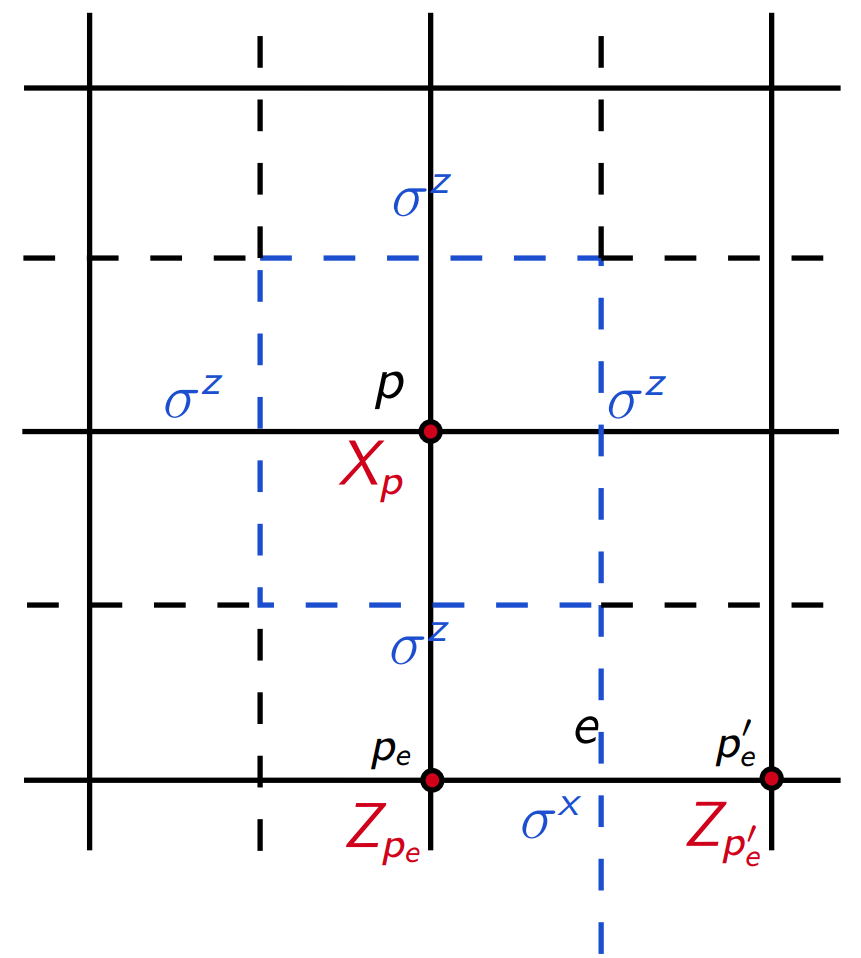
\includegraphics[width=\textwidth]{images/z2_gauge_theory/dual_lattice.tex}
    \end{subfigure}
    \caption{Wegner  duality mapping of the $\mathbb{Z}_2$ lattice gauge theory to a $\mathbb{Z}_2$ spin (Ising) model. The dotted lines with link gauge variables denotes the original $\mathbb{Z}_2$ gauge theory lattice and the solid lines with vertex spin variables represents the dual lattice.}
    \label{dual_lattice}
\end{figure}
%%% FIG %%%
\section{Wegner duality}
In the context of the $\mathbb{Z}_2$ lattice gauge theory, we map the gauge theory to a spin model via the Wegner duality mapping for the following reasons:
\begin{itemize}
    \setlength{\itemsep}{0.1em}
    \item it eliminates the redundant and unphysical gauge degrees of freedom by mapping it to a spin model with a global $\mathbb{Z}_2$ symmetry. Therefore, there are no local Gauss' law constraints.
    \item it maps the interacting terms in the $\mathbb{Z}_2$ lattice gauge theory into the non-interacting terms in the $\mathbb{Z}_2$ spin model and vice-versa, resulting in the inversion of the coupling constants. 
    \item it realizes the same algebra between the gauge and spin degrees of freedom.
\end{itemize}
More precisely, the Wegner duality is defined by the following
dual mapping:
\begin{equation}
    \sigma^x_{\: e} = \sigma^x_{\: p_e p'_e} \longrightarrow Z_{p_e} Z_{p'_e}, \qquad\qquad \prod_{e \: \in \: p} \sigma^z_{\:e} = B_p \longrightarrow X_p.
\end{equation}
where $X_p$ and $Z_p$ are the new spin degrees of freedom on the dual lattice. Furthermore, as mentioned earlier, they satisfy the same algebra, and it is straightforward to show that
\begin{equation}
    X_p^2 = B_p^2 = \mathds{1}, \qquad \{X_p, Z_p\} = \mathds{1}, \qquad [X_{p_e}, Z_{p'_e}] = 0 \text{  if } p_e \neq p'_e   
\end{equation} 
The Hilbert space on which $X$, $Z$ operators act is on a set of spins placed at the centre of the plaquettes at $p$. This is also shown in Fig. \ref{dual_lattice} where the $\mathbb{Z}_2$ gauge theory lattice is represented by dotted lines with link degrees of freedom, and the dual lattice is represented by the solid lines with vertex degrees of freedom.

Following the same dual transformation, the dual Hamiltonian becomes
\begin{equation}
    \hat{H} = -J \sum_p X_p - h \sum_e Z_{p_e} Z_{p'_e}
    \label{tfim}
\end{equation}
which is nothing but the transverse field Ising model (TFIM) with interchanged couplings. However, for the duality to strictly hold, the constraints must also be mapped accordingly. The Gauss' law constraint Eq. \eqref{gausslaw} of the original theory is automatically satisfied since 
\begin{equation}
    \hat{G_v} = \prod_{e \:\in\: +_v} \sigma^x_{\: e} = \!\!\!\!\!\!\! \prod_{\expval{p_e, \: p'_e} \: \in \: \Box_v} \!\!\!\!\!\!  Z_{p_e} Z_{p'_e} \equiv \mathds{1}
\end{equation}
where the last equality follows because each $Z_{p_e}$ term appears twice. However, the constraint due to periodic boundary conditions isn't trivially satisfied and instead forces
\begin{equation}
    \prod_p B_p = \prod_p X_p \stackrel{!}{=} \mathds{1}
    \label{singlet}
\end{equation}
which is a constraint on the Hilbert space of the dual model, and is known as the \textbf{singlet constraint}. We thus conclude that the dual theory is a quantum Ising model (or TFIM) Eq. \eqref{tfim} with the singlet constraint Eq. \eqref{singlet}.
\section{Quantum to classical correspondence}
The Ising model is one of the simplest spin models studied extensively in condensed matter physics. However, in the presence of a transverse field Eq. \eqref{tfim} (represented by the $X_p$ operator), the Hamiltonian is not trivially diagonalizable in the $Z$ basis $\{\ket{\uparrow}, \ket{\downarrow} \}$ anymore. Solving this quantum problem directly is somewhat difficult. Therefore, we invoke of the principle of quantum to classical correspondence, which connects the partition functions of the a $d$-dimensional quantum system to a $d+1$-dimensional classical statistical mechanical system via a path integral approach~\cite{suzuki}. The Path Integral Monte Carlo (PIMC) method then uses classical Monte Carlo simulations to calculate the physically relevant quantities of the quantum system.
\subsection{Imposing the singlet constraint ``exactly''}
As noted in the previous section, the $\mathbb{Z}_2$ gauge theory with periodic boundary conditions is dual to the singlet Ising model with nearest neighbor interactions,

\begin{equation}
    \hat{H} = \underbrace{-J \sum_i X_i}_{H_T} - \underbrace{h \sum_{\expval{i, \:j}} Z_{i} Z_{j}}_{H_I}, \qquad \prod_i X_i = \mathds{1}
\end{equation} 
where $H_I$ denotes the Ising interaction part, and $H_T$ denotes the transverse field part of the Hamiltonian. Let us first note that
\begin{equation}
    \hat{F} \equiv \prod_i X_i \implies \hat{F}^2 = \mathds{1}.
    \label{flipoperator}
\end{equation}  
Thus, we can define the projection operator on the singlet subspace as
\begin{equation}
    \hat{P} = \frac{1}{2}(\mathds{1} + \hat{F}) = \frac{1}{2} \sum_{\mu' \: \in \: \{0, 1\}} \hat{F}^{\mu'}
\end{equation}
The partition function of the singlet Ising model can thus be written as a trace over the singlet-basis states $\{\hat{P} \ket{\{\sigma\}} \}$ where $\ket{\{\sigma\}} = \ket{\sigma_1 \: \sigma_2 \: \ldots \sigma_{N_x}}$ are the $Z$-basis product states $\sigma_i \: \in \: \{\pm 1\}$.
\begin{equation}
    \mathcal{Z} = \tr e^{-\beta \hat{H}} = \sum_{\{\sigma\}} \mel{\{\sigma\}}{\hat{P} \: e^{-\beta \hat{H}} \: \hat{P}}{\{\sigma\}}
\end{equation}
where $\sum_{\{\sigma\}}$ denotes a sum over all $2^{N_x}$ different lattice configurations. Further, since $\{\hat{P} \ket{\{\sigma\}} \}$ now form the singlet-basis, their outer products defines the singlet-identity operator $\mathds{1}_s$,
\begin{equation}
    \mathds{1}_s = \sum_{\{\sigma\}} \hat{P} \ket{\{\sigma\}} \bra{\{\sigma\}} \hat{P} = \frac{1}{4} \sum_{\{\sigma\}, \mu', \lambda'} \hat{F}^{\lambda'} \ket{\{\sigma\}} \bra{\{\sigma\}} \hat{F}^{\mu'}  
\end{equation}
Since $\hat{F}^{\mu'} = (\prod_i X_i)^{\mu'}$ flips all the spins $\{\sigma\} \longrightarrow \{-\sigma\}$ or leaves them invariant $\{\sigma\} \longrightarrow \{+\sigma\}$ for the cases ${\mu'} = -1$ and ${\mu'} = +1$, respectively. Therefore, an alternate representation of its action on the basis states is $\hat{F}^{\mu'} \ket{\{\sigma\}} = \ket{\{\mu \: \sigma\}}$ where $\mu'= (-1)^{\mu} \implies \mu \: \in \: \{\pm 1\}$. The singlet-identity (ignoring the $1/4$ factor) can then be rewritten as
\begin{equation}
    \mathds{1}_s = \sum_{\mu, \:\lambda \: \in \: \{\pm 1\}} \ket{\{\lambda \: \sigma\}} \bra{\{\mu \: \sigma\}}
\end{equation}
We will now begin the path integral procedure by slicing the inverse temperature into tiny pieces of width $\Delta \tau$ such that $\beta = N_\tau \Delta \tau$. The Boltzmann exponential factor can then be written as
\begin{equation}
    e^{-\beta \hat{H}} = \underbrace{e^{-\Delta \tau \hat{H}} \: e^{-\Delta \tau \hat{H}} \: e^{-\Delta \tau \hat{H}} \ldots e^{-\Delta \tau \hat{H}}}_{N_\tau \text{ times}}
\end{equation}  
and we can insert a singlet-identity between each exponential factor. We will also drop the hats for notational convenience
\begingroup
\allowdisplaybreaks
\begin{align}
    \mathcal{Z} &= \sum_{\{\sigma\}, \:\mu, \:\lambda} \mel{\{\mu \: \sigma\}}{e^{-\beta {H}} e^{-\beta {H}} \ldots e^{-\beta {H}} }{\{ \lambda \: \sigma\}} \nonumber \\
    &= \sum_{\{\sigma_0\}, \:\mu_0, \:\lambda_0} \mel{\{\mu_0 \: \sigma_0\}}{ e^{-\beta {H}} \:\mathds{1}_s\: e^{-\beta {H}} \:\mathds{1}_s\: \ldots \mathds{1}_s\: e^{-\beta {H}} \: }{\{ \lambda \: \sigma_0\}} \nonumber \\
    &= \qty(\prod_{l=0}^{N_\tau-1} \sum_{\{\sigma_l\}, \mu_l, \lambda_l}) \prod_{l=0}^{N_\tau-1} \mel{\{\mu_{l+1} \sigma_{l+1}\}}{e^{-\Delta \tau H}}{\{\lambda_{l} \sigma_l\}}
    \label{partitionfn}
\end{align}
\endgroup
where the $2N_\tau$ objects $\mu_l, \: \lambda_l$ each run over $\{\pm 1\}$, with $\mu_{N_\tau} = \mu_0$, $\lambda_{N_\tau} = \lambda_0$, and $\ket{\{\sigma_{N_\tau}\}} = \ket{\{\sigma_{0}\}}$. This new index $l$ adds an additional dimension to our problem, and acts like an imaginary time index, with the matrix elements acting like infinitesimal transition amplitudes between imaginary time layers. All the calculations till here have been exact without considering any limits. We now utilize the Trotter product formula to assert that in the limit $N_\tau \to \infty$ or $\Delta \tau \to 0$, the exponential can be decomposed as follows:
\begin{equation}
    e^{-\Delta \tau H} = e^{-\Delta \tau (H_I + H_T)} = e^{-\Delta \tau H_I} e^{-\Delta \tau H_T} + \mathcal{O}(\Delta \tau^2) 
\end{equation}
and we effectively ignore the higher order terms, introducing our first approximation. This approximation gets better as $N_\tau$ grows larger. Let us begin by analyzing the matrix elements in the product in Eq. \eqref{partitionfn}.
\begingroup
\allowdisplaybreaks
\begin{align}
    \mel{\{\mu_{l+1} \sigma_{l+1}\}}{e^{-\Delta \tau H}}{\{\lambda_{l} \sigma_l\}} &\approx \mel{\{\mu_{l+1} \sigma_{l+1}\}}{e^{-\Delta \tau H_T} e^{-\Delta \tau H_I}}{\{\lambda_{l} \sigma_l\}} \nonumber\\
    & = \underbrace{\mel{\{\mu_{l+1} \sigma_{l+1}\}}{e^{-\Delta \tau H_T}}{\{\lambda_l \sigma_l\}}}_{M_{l+1, l}} e^{-\Delta \tau H_I[\{\mu_l \sigma_l\}]}
    \label{Ml+1,l}
\end{align}
\endgroup
where $H_I[\{\mu_l \sigma_l\}]$ is the Ising configuration at the imaginary time layer $l$  
\begingroup
\allowdisplaybreaks
\begin{align}
    H_I[\{\mu_l \sigma_l\}] &= -h \sum_i \mu_l \sigma_l(i) \mu_l \cdot \sigma_l (i+1) \nonumber \\
    &= -h \sum_i \sigma_l(i) \sigma_l (i+1) = H_I[\{\sigma_l\}]
    \label{isingterm}
\end{align}
\endgroup
since $\mu_l^2 = 1$, and $H_I[\{\sigma_l\}]$ is a classical Ising interaction without any operators. Let us now analyze the leftover matrix element $M_{l+1, \:l}$ in Eq.~\eqref{Ml+1,l}
\begingroup
\allowdisplaybreaks
\begin{align}
    M_{l+1, \: l} &= \mel{\{\mu_{l+1} \sigma_{l+1}\}}{e^{-\Delta \tau H_T}}{\{\lambda_l \sigma_l\}} = \mel{\{\mu_{l+1} \sigma_{l+1}\}}{e^{+ J\Delta \tau \sum_{i} X_i}}{\{\lambda_l \sigma_l\}} \nonumber \\
    & = \prod_{i} \mel{\mu_{l+1} \sigma_{l+1}(i)}{e^{J \Delta \tau X_i}}{\lambda_{l} \sigma_l(i)} \nonumber \\
    & = \prod_{i} \mel{\mu_{l+1} \sigma_{l+1}(i)}{\cosh(J \Delta \tau) \mathds{1} + \sinh(J \Delta \tau)X_i }{\lambda_{l} \sigma_l(i)} \nonumber \\
    & = \prod_{i} C_l(i)
    \label{matrixelement}
\end{align}
\endgroup
The matrix element $C_l(i)$ can further be evaluated as follows: we can write it as an arbitrary function $C_l(i) = A e^{K(\mu_{l+1}\lambda_l \: \sigma_{l+1}(i)\sigma_{l}(i))}$ where we don't yet know the constants $A$ and $K$. However, due to the structure of the matrix element,
\begin{equation}
    C_l(i) = 
    \begin{cases}
    \cosh(J \Delta \tau), & \text{ if } \mu_{l+1}\lambda_l \: \sigma_{l+1}(i)\sigma_{l}(i) = +1 \\
    \sinh(J \Delta \tau), & \text{ if } \mu_{l+1}\lambda_l \: \sigma_{l+1}(i)\sigma_{l}(i) = -1       
    \end{cases}
    \label{cases}
\end{equation}
From the postulated form of $C_i(l)$ and Eq. \eqref{cases}, we can infer that 
\begingroup
\allowdisplaybreaks
\begin{align}
A e^{K} = \cosh(J \Delta \tau), \qquad A e^{-K} = \sinh(J \Delta \tau)
\end{align}
\endgroup
By dividing and multiplying the two equalities above, we obtain the values of the constants
\begingroup
\allowdisplaybreaks
\begin{align}
A = \sqrt{\frac{1}{2} \sinh(2 J\Delta \tau )}, \qquad K = -\frac{1}{2} \ln \tanh (J \Delta \tau)
\label{constants}
\end{align}
\endgroup
Therefore, the matrix element $M_{l+1, \:l}$ in Eq. \eqref{matrixelement} can be written in the following form
\begin{equation}
    M_{l+1, \: l} = A^{N_x} \exp \qty[(\mu_{l+1} \lambda_l)\sum_i K \sigma_{l+1}(i) \: \sigma_{l}(i)]
    \label{finalmel}
\end{equation}
Further, we define 
\begin{equation}
    Y = h \Delta \tau
\end{equation}
Combining eqns.~\eqref{finalmel},~\eqref{isingterm}, and~\eqref{partitionfn}, we can write the partition function as 
\begingroup
\allowdisplaybreaks
\begin{align}
    \mathcal{Z} = \qty(\prod_{l=0}^{N_\tau-1} \sum_{\{\sigma_l\}, \mu_l, \lambda_l}) e^{-S'[\sigma, \lambda, \mu]}
\end{align}
\endgroup
where 
\begingroup
\allowdisplaybreaks
\begin{align}
    S'[\sigma, \lambda, \mu] = - \sum_l \qty[\mu_{l+1} \lambda_l \sum_i K \: \sigma_{l+1}(i) \: \sigma_{l}(i)] - \sum_l\qty[\sum_i Y \: \sigma_l(i) \sigma_l (i+1)]
\end{align}
\endgroup
The final partition function expression only contains the product $\mu_{l+1} \lambda_l = \xi_l$. Therefore, we can replace sum over $\mu_l, \lambda_l \: \in \: \{\pm 1\}$ for each $l$ with a sum over $\xi_l \: \in \: \{\pm 1\}$. Therefore, apart from an overall factor, the partition function looks like 
\begin{equation}
    \mathcal{Z} = \qty(\prod_{l=0}^{N_\tau-1} \sum_{\{\sigma_l\}, \:\xi_l}) e^{-S'[\sigma, \: \xi]}
    \label{abcd}
\end{equation}
where 
\begingroup
\allowdisplaybreaks
\begin{align}
    S'[\sigma, \xi] & = - \sum_l \xi_l \underbrace{\qty[\sum_i K \: \sigma_{l+1}(i) \: \sigma_{l}(i)]}_{H_\tau(l+1, l)} - \sum_l \underbrace{\qty[\sum_i Y \: \sigma_l(i) \sigma_l (i+1)]}_{H_I(l)} \nonumber \\
    & = - \sum_l \xi_l \: H_\tau(l+1, l) - \sum_l H_I(l)
\end{align}
\endgroup
If we now write down the partition function and perform a sum over $\xi_l \: \in \: \{\pm 1\}$ in Eq.~\eqref{abcd},
\begingroup
\allowdisplaybreaks
\begin{align}
    \mathcal{Z} & = \prod_{l=0}^{N_\tau-1} \qty[\sum_{\{\sigma_l\}} e^{\sum_l H_I(l)} \qty( \sum_{\{\xi_l \: \in \: \pm 1\} } e^{\sum_l \xi_l \: H_\tau(l+1, l)})] \nonumber \\
    & = \prod_{l=0}^{N_\tau-1} \qty[\sum_{\{\sigma_l\}} e^{\sum_l H_I(l)} \qty( \prod_{l=0}^{N_\tau - 1} \qty(\sum_{\{\xi_l \: \in \: \pm 1\} } e^{\xi_l \: H_\tau(l+1, l)}))]   \nonumber \\
    & = \prod_{l=0}^{N_\tau-1} \qty[\sum_{\{\sigma_l\}} e^{\sum_l H_I(l)} \qty( \prod_{l=0}^{N_\tau - 1} \cosh \qty(H_\tau(l+1, l)))]   \nonumber \\
    & = \prod_{l=0}^{N_\tau-1} \qty[\sum_{\{\sigma_l\}} e^{\sum_l H_I(l)} \: e^{\sum_l \ln \cosh \qty(H_\tau(l+1, l))}]   \nonumber \\
    & = \qty(\prod_{l=0}^{N_\tau-1} \sum_{\{\sigma_l\}}) e^{-S[\sigma]}
\end{align}
\endgroup
where the effective classical action (with the singlet constraint imposed) is given by
\begin{equation}
    S[\sigma] = -Y\sum_l \sum_i \sigma_l(i) \: \sigma_l(i+1) - \sum_l \ln \cosh \qty[K \sum_i \sigma_{l+1}(i) \: \sigma_{l}(i)]
    \label{classicalaction}
\end{equation} 
%%% FIG %%%
\begin{figure}[t!]
    \centering
    \begin{subfigure}[b]{0.8\textwidth}  %keep total sum <1 to show in same line
        \centering
        \includegraphics[width=\textwidth]{images/z2_gauge_theory/quantumtoclassical.tex}
    \end{subfigure}
    \caption{Mapping of the $d=1$ quantum model to a $(d+1) = (1+1)$-dimensional classical Ising model.}
    \label{}
\end{figure}
%%% FIG %%%
If we start with a $d$-dimensional quantum Ising model, the quantum to classical correspondence maps it to a $d+1$-dimensional generalized classical Ising model, where the spatial interactions contains standard pairwise terms $\sim \sigma_l(i) \: \sigma_l(i)$, but the layer interactions are governed by a $\sim \ln \cosh (\sigma_{l+1}(i) \: \sigma_{l}(i))$. This classical model can then be simulated using the classical Metropolis Monte Carlo algorithm. For the purposes of this thesis, we will be studying the classical analog of the singlet Ising model (Eq. \eqref{classicalaction}) in $(1 + 1)d$ and the relevant physical observables using Monte Carlo simulations.

\subsection{Alignment observable and the subsystem symmetry}\label{alignmentsection}
Let us begin by looking at a particularly interesting local observable which appears inside the $\ln \cosh$ term in the classical action Eq. \eqref{classicalaction}. We call this observable as the alignment observable 
\begin{equation}
    A(l) \equiv \frac{1}{N_x} \sum_{i=0}^{N_x-1} \sigma_i(l) \sigma_i(l+1) = \frac{1}{N_x}\qty(N_a(l) - N_o(l))
\end{equation}
%%% FIG %%%
\begin{figure}[t!]
    \centering
    \begin{subfigure}[b]{0.6\textwidth}  %keep total sum <1 to show in same line
        \centering
        \includegraphics[width=\textwidth]{images/z2_gauge_theory/alignmentflip.tex}
    \end{subfigure}
    \caption{The action of the alignment flip operation $\hat{F}(l)$ on the individual spins and the alignment observable $A(l)$. The blue links denote an aligned pair, and the orange links denote an oppositely aligned pair. The links flip on the application of $\hat{F}(l)$, also flipping the value of $A(l)$ and $A(l-1)$.}
    \label{alignflip}
\end{figure}
%%% FIG %%%
\FloatBarrier
where $N_a$ denotes the number of aligned pairs and $N_o$ denotes the number of oppositely aligned pairs. This observable effectively measures the \textit{alignment} between the spins of layers $l$ and $l+1$. In terms of the local alignment observables, the classical action for a $(1+1)$-dimensional classical model can be rewritten as
\begin{equation}
    S[\sigma] = -Y\sum_{l=0}^{N_\tau-1} \sum_{i=0}^{N_x-1} \sigma_l(i) \: \sigma_l(i+1) - \sum_{l=0}^{N_\tau-1} \ln \cosh \qty[K N_x A(l)]
    \label{2daction}
\end{equation}
The alignment observable transforms in a special way under a transformation, which makes it worth tracking. 

Consider a transformation which flips the spins along a particular layer $l$. Although we aren't formally working with quantum objects right now, we can still define the transformation via a local ``operator'' 
\begin{equation}
    \hat{F}(l) \equiv \prod_{i=0}^{N_x-1} \hat{X}_{i, \: l}
    \label{alignmentflip}
\end{equation}
where the $\hat{X}_{i, \: l}$ flips the classical spin variables $\sigma_{l}(i) \longrightarrow -\sigma_{l}(i)$. Since it only flips the spins along the layer $l$, 
\begingroup
\allowdisplaybreaks
\begin{align}
    &A(l) \longrightarrow \frac{1}{N_x} \sum_{i=0}^{N_x-1} [-\sigma_i (l)] \sigma_i(l+1) = -A(l) \nonumber \\
    &A(l-1) \longrightarrow \frac{1}{N_x} \sum_{i=0}^{N_x-1} \sigma_i (l-1) [-\sigma_i(l)] = -A(l-1)
\end{align}
\endgroup
it flips the alignments of the layers $l$ and $l-1$ (Fig. \ref{alignflip}). Therefore, it's also commonly referred to as an \textit{alignment flip} operation. However, the classical action (Eq. \eqref{2daction}) contains terms which remain agnostic under the above transformation 
\begin{itemize}
    \setlength{\itemsep}{0.1em}
    \item Spatial interaction: $\displaystyle [-\sigma_l(i)] [-\sigma_l(i+1)] = \sigma_l(i) \: \sigma_{l}(i+1)$.
    \item Temportal interaction: $\displaystyle \ln \cosh[K N_x (-A(l))] = \ln \cosh [K N_x A(l)]$ 
\end{itemize}
Therefore, the action remains invariant under the alignment flip operator,
\begin{equation}
    S[\sigma] \xlongrightarrow{\text{Alignment Flip } \hat{F}(l)} S[\sigma]
    \label{actioninvariant}
\end{equation}
and the alignment flip operator $\hat{F}(l)$ is referred to as a \textit{subsystem symmetry}. 

This also implies that configuration space states with positive and negative values of the alignment observable would be equally probable in a stochastic simulation such as Monte Carlo. Therefore, on average, $\expval{A(l)} \stackrel{!}{=} 0 \:\: \forall \: l$, and this quantity can be used as a proxy for ensuring that our effective classical model is indeed simulating the singlet constrained physics of the quantum model.

\section{Naive Metropolis Monte Carlo simulations}
In this section, we will discuss a direct Metropolis Monte Carlo implementation of the $(1+1)d$ generalized classical Ising model in Eq. \eqref{2daction}. We have already outlined the major details of the Metropolis algorithm in Chapter \ref{chap:1}. The Metropolis algorithm only consists of spin flip proposals on the $(1+1)d$ lattice. As we'll see later, this straightforward but naive implementation doesn't give the correct equilibration behavior and doesn't simulate the correct physics of the problem.

In quantum Monte Carlo simulations such as these, we usually keep $\Delta \tau = 1$, i.e. $\beta = N_\tau$, and the ground state properties of the system are studied by making the number of sites on the imaginary time axes as large as possible $N_\tau \to \infty$. As mentioned in the last section, we are particularly interested in tracking the Monte Carlo average of  the alignment observables which act as an indicator of a good simulation. We perform the simulation over increasing lattice sizes $N_x$ and an increasing number of Monte Carlo sweeps to understand the dependence on the simulation results on these parameters.

For the simulations, we use the following parameters
\begin{itemize}[label={}]
    \setlength{\itemsep}{0.1em}
    \item \texttt{spatial lattice size } $N_x \in \{ \texttt{2, 3, 4 $\ldots$, 20} \}$  
    \item \texttt{no of sampling sweeps } $N_\text{samp} \in \{\texttt{2.0e4, 6.0e4, 1.0e5, $\ldots$, 2.6e5, 3.0e5} \}$
    \item \texttt{imaginary time lattice size } $N_\tau = $ \texttt{40}, \: $\Delta \tau = $ \texttt{1.0}
    \item \texttt{coupling constants} $K,\: Y = $ \texttt{1.0}
\end{itemize}

%%% FIG %%%
\begin{figure}[t!]
    \centering
    \begin{subfigure}[b]{0.47\textwidth}
        \centering
        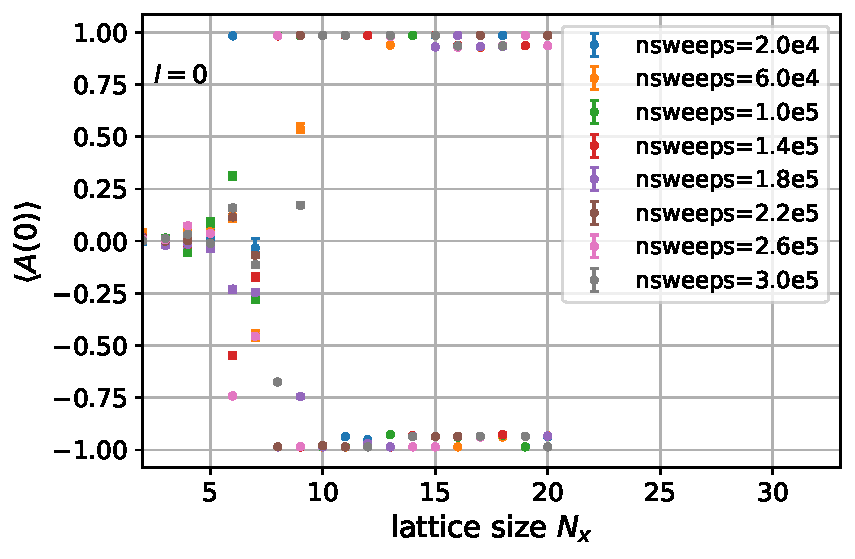
\includegraphics[width=\textwidth]{images/expval(A_l)_vs_N_x/A vs N_x (l=0).pdf}
        \caption{$\expval{A(0)} \text{ vs } N_x$}
    \end{subfigure}
    \hspace{1em}  %\hfill
    \begin{subfigure}[b]{0.47\textwidth}
        \centering
        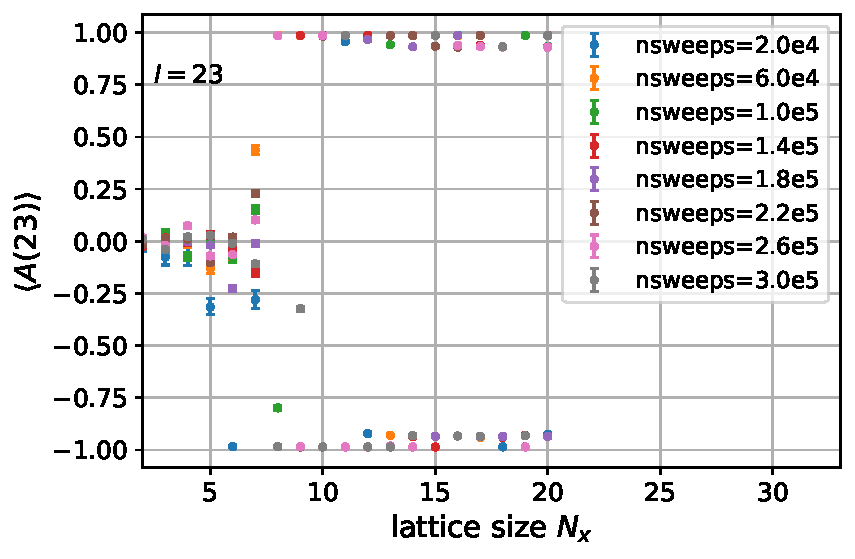
\includegraphics[width=\textwidth]{images/expval(A_l)_vs_N_x/A vs N_x (l=23).pdf}
        \caption{$\expval{A(23)} \text{ vs } N_x$}
    \end{subfigure}
    \caption{$\expval{A(l)}$ for different values of $l$.}
    \label{SSB}
\end{figure}
%%% FIG %%%
\subsection{Subsystem symmetry breaking}
As seen in Fig.~\ref{SSB}, the results show weak dependence on the number of Monte Carlo sweeps as the system always explores the same region of the configuration space, independent of the number of sweeps. However, above a certain lattice size, i.e., $N_x \sim 10$, the expectation value of the alignment observable gets frozen to $\pm 1$. This effect is independent of the layer chosen as all layers are identical to each other, and is also verified in Fig.~\ref{differentlayer_sameMCsweeps} by plotting the results for two different layers.
%%% FIG %%%
\begin{figure}[!htb]
    \centering
    \begin{subfigure}[b]{0.5\textwidth}
        \centering
        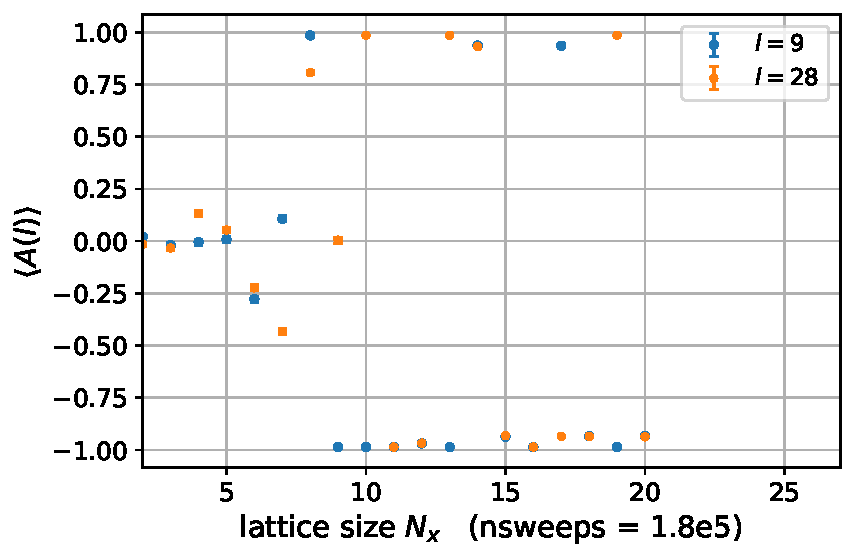
\includegraphics[width=\textwidth]{images/expval(A_l)_vs_N_x/A vs N_x (nsweeps=1.8e5).pdf}
    \end{subfigure}
    \caption{$\expval{A(l)}$ vs $N_x$ for two different layers $l_1 = 9,\: l_2 = 28$ ran over \texttt{nsweeps = 1.8e5}.}
    \label{differentlayer_sameMCsweeps}
\end{figure}
%%% FIG %%%
\FloatBarrier
The freezing of the alignment value to $\expval{A(l)} \neq 0$ indicates that the minima of the action $S[\sigma]$ gets extremely deep on the opposite sides of the configuration space which leads to a high energy barrier between the $A(l)= - 1$ and $A(l) = +1$ sides of the configuration space.

The breaking of this subsystem symmetry gives us the first indication that a naive implementation of the Metropolis algorithm cannot give us the correct equilibration behavior of this system.

\subsection{Autocorrelation function}
Another quantity which is shown to give undesired results with the onset of subsystem symmetry breaking is the autocorrelation function of the alignment observable $A(l)$. For the notational convenience, we briefly switch to writing $A(l)$ as $A_l$. For the observable $A_l$, the autocorrelation function is computed as follows
\begin{equation}
    \text{Autocorr}[A_l] = \frac{\expval{A_l(k) A_l(k+T)}}{\expval{A_l(k)^2}} = \frac{1}{N-T} \sum_{k=0}^{N-T-1} \frac{A_l(k) \cdot A_l(k+T)}{\expval{A_l(k)^2}}
\end{equation} 
where the average is taken over the first $N-T$ measurements, i.e.
\begin{equation}
    \langle{A_l(k)^2}\rangle = \frac{1}{N-T} \sum_{k=0}^{N-T-1} [A(k)]^2
\end{equation}
One might notice that this definition of autocorrelation function looks slightly different. This is because we have forced $\expval{A_l} = 0$, since that is the general expectation when the desired subsystem symmetry is present in the system. If we don't force $\expval{A_l} = 0$, we would obtain autocorrelation values for the system oscillating in one of the minima wells, which is an undesirable quantity for us.

In the following simulation, we have set \texttt{nsweeps = 2.0e4}, $N_x = $ \texttt{20}, $N_\tau = $ \texttt{40}, $\Delta \tau = $ \texttt{1.0}, and the autocorrelations are computed for $T \in \{ $ \texttt{1, 2, $\ldots$, 3000} $\}$.     
%%% FIG %%%
\begin{figure}[!htb]
    \centering
    \begin{subfigure}[b]{0.5\textwidth}
        \centering
        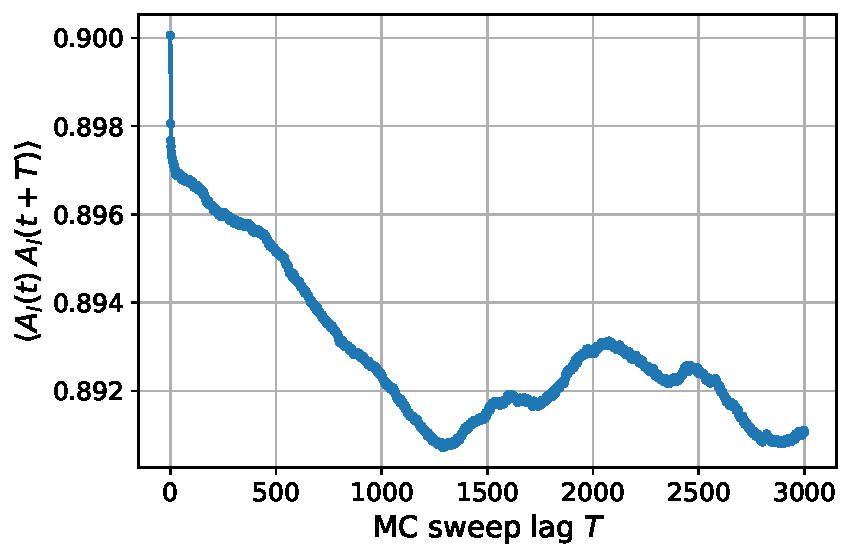
\includegraphics[width=\textwidth]{images/misc/autocorrfn_singlet.pdf}
    \end{subfigure}
    \caption{Autocorrelation function $\expval{A_l(k) A_l(k+T)}$.}
    \label{autocorrs_singlet}
\end{figure}
%%% FIG %%%
\FloatBarrier
In Fig.~\ref{autocorrs_singlet}, we see that the autocorrelation function stays nearly constant $\approx 0.89$ even for $T = 3000$, which implies that autocorrelation time $\tau \to \infty$ for the observables $A(l)$. Hence, once the system gets stuck in one of the $A(l) \pm 1$ minima wells, it almost never gets the chance to escape to the other side of the configuration space. 

Therefore, a naive Metropolis algorithm implementation with single spin flips to govern the Monte Carlo dynamics is not sufficient to simulate our effective classical system with subsystem symmetries (which is a direct consequence of the singlet constraint).

\section{Restoring the subsystem symmetry}
In the previous section, we were able to conclusively arrive at the fact that single spin flip Metropolis Monte Carlo simulations are insufficient for exploring the $(1+1)d$ generalized classical Ising model. Due to the freezing of the alignment measurements, the Markov chain describing the single spin flip Metropolis simulation is found to not be ergodic. 

This type of a symmetry breaking also occurs in the classical $\mathbb{Z}_2$ Ising model (without any $\ln \cosh$ terms), where the ferromagnetic phase appears as a $\mathbb{Z}_2$ symmetry-broken phase and describes the actual physics instead of being a problem. However, in our case, subsystem symmetry breaking is an obstacle and its preservation is crucial since we want our original quantum model to remain in the singlet sector of the Hilbert space.

\subsection{Alignment flips as Metropolis proposal moves}
The root cause of subsystem symmetry breaking is the inability of the standard Metropolis Monte Carlo to explore the entire configuration space. This is because the two equally accessible regions have a strong energy barrier between them, preventing states of positive (negative) alignment to tunnel to states of negative (positive) alignment.

One of the possible ways to restore this symmetry is by utilizing the special properties of the alignment flip operation Eq.~\eqref{alignmentflip} defined in Section~\ref{alignmentsection}. The alignment flip operation fixes the problem of alignment freezing by forcefully flipping the alignment of a layer, thereby introducing a new channel for connecting positively and negatively aligned regions of the configuration space which was previously inaccessible.

Another interesting feature of the alignment flip operation is that it leaves the effective classical action $S[\sigma]$ invariant Eq.~\eqref{actioninvariant}. As a consequence, if the alignment flip operation is introduced as a Metropolis proposal move, then it is an always accepted move since $\Delta S = 0$ always. Therefore, we \textit{propose} that the \textit{modified Metropolis algorithm} is a combination of both random spin flip proposals as well as random alignment flip operations. More precisely, a single Monte Carlo sweep of this modified algorithm is defined as follows,
\begin{itemize}
    \setlength{\itemsep}{0.1em}
    \item $N_x N_\tau$ random spin flip proposals on the $(1+1)d$ lattice.   
    \item $\lfloor N_\tau/f \rfloor$ random alignment flips.
\end{itemize}
where $f \in \mathbb{R}^+$ tunes the ratio of number of random alignment flips to the number of random spin flip proposals. We expect small values of $f \sim \mathcal{O}(1)$ should be enough to restore the subsystem symmetry in our simulations.

\subsection{Algorithm}
We will now discuss an algorithmic implementation by including both random alignment flip and random spin flip proposals into the Monte Carlo simulation, i.e., ${f N_x}$  random spin flip proposals followed by one random alignment flip.

\begin{algorithm}{singlet-metropolis}
    \> define $\sigma[N_x ,N_\tau];$ \\
    \> \text{initialize spins} $\sigma[i, l]$;\\
    \> \text{define weighted alignment array} $\varepsilon[N_\tau];$ \\
    \> \text{initialize } $\varepsilon[l] = \sum_i K_i \sigma_i(l+1) \sigma_i(l), \quad\forall\: l;$ \\
    \> \texttt{// Metropolis updates} \\
    \>{\bf for} $n \in \{1, 2, \ldots N_\text{samp}\}$ \\
    \>{\bf begin}\\
    \>\> \texttt{// Single Monte Carlo step} \\
    \>\>{\bf for} $m \in \{1, 2, \ldots N_x \cdot N_\tau \}$ \\
    \>\>{\bf begin}\\
    \>\>\> \texttt{// Random spin flip proposal} \\
    \>\>\> \text{choose site (random, sequential) }$:=(i_0, l_0)$;\\
    \>\>\> define $\varepsilon'_{l_0}, \:\:
    \varepsilon'_{l_0 - 1}; $\\
    \>\>\> define $\Delta S, \:\: \Delta S_x, \:\: \Delta S_t;$\\
    \\
    \>\>\> $\varepsilon'_{l_0-1} = \varepsilon[l_0-1] + 2K_{i_0}\cdot\sigma(i_0, l_0)\cdot\sigma(i_0, l_0-1);$\\
    \>\>\> $\varepsilon'_{l_0}\:\:\:\: = \varepsilon[l_0] \:\:\:\:\quad + 2K_{i_0}\cdot\sigma(i_0, l_0)\cdot\sigma(i_0, l_0+1);$\\
    \\
    \>\>\> $\Delta S_x = 2\Delta \tau \cdot h_{i_0} \cdot \sigma(i_0, l_0) \cdot [\sigma(i_0-1,l_0) + \sigma(i_0+1,l_0)];$ \\
    \>\>\> $\Delta S_t = \ln \qty[\cosh(\varepsilon[l_0])/\cosh(\varepsilon'_{l_0})] + \ln\qty[\cosh(\varepsilon[l_0-1])/\cosh(\varepsilon'_{l_0-1})] ;$ \\
    \>\>\> $\Delta S = \Delta S_x + \Delta S_t ;$ \\ 
    \\
    \>\>\> define $p = $ random number; \\
    \>\>\>{\bf if} $p < \exp(-\Delta S)$\\  
    \>\>\>{\bf begin}\\
    \>\>\>\> $\varepsilon[l_0 - 1] = \varepsilon'_{l_0-1}$; \\
    \>\>\>\> $\varepsilon[l_0] \:\:\:\:\quad =  \varepsilon'_{l_0}$; \\
    \>\>\>\> $\sigma[i_0, l_0] = (-1)\cdot \sigma[i_0, l_0];$\\
    \>\>\>{\bf end}\\
    \\
    \>\>\> \texttt{// Random alignment flip moves} \\
    \>\>\> {\bf if} $m$ \texttt{\%} $f N_x \texttt{==0}$  \\
    \>\>\> {\bf begin} \\
    \>\>\>\> \text{choose random layer } $:= \: l$ \\
    \>\>\>\> {\bf for } $i \in \{1, 2, \ldots N_x\}$ \\
    \>\>\>\>{\bf begin} \\
    \>\>\>\>\> $\sigma[i, l] = (-1)\cdot \sigma[i, l];$\\
    \>\>\>\>{\bf end}\\    
    \>\>\>\> $\varepsilon[l - 1] = - \varepsilon[l - 1]$; \\
    \>\>\>\> $\varepsilon[l] \:\:\:\:\quad =  - \varepsilon[l]$; \\
    \>\>\> {\bf end}\\

    \>\>{\bf end}\\
    \>{\bf end} \\
\end{algorithm}
We implement the above algorithm in \texttt{C++} and parallelize it using the \texttt{mpi4py} package in \texttt{Python}. 
\subsection{Results with alignment flips}
This section reviews the results obtained from the singlet Metropolis Monte Carlo simulation with alignment and spin flip moves.~\\~\\
\textbf{Simulation parameters}
\begin{itemize}[label={}]
    \setlength{\itemsep}{0.1em}
    \item \texttt{alignment flip fraction $f = $ 2.0}
    \item \texttt{spatial lattice size } $N_x \in \{ \texttt{2, 4, 6 $\ldots$, 32} \}$  
    \item \texttt{no of sampling sweeps $N_\text{samp} = $ 5.0e4} 
    \item \texttt{imaginary time lattice size } $N_\tau = $ \texttt{40}, \: $\Delta \tau = $ \texttt{1.0}
    \item \texttt{coupling constants} $K, Y = $ \texttt{1.0} 
\end{itemize}
The simulations are performed both with and without alignment flips and the results of the expectation values of $A(l)$ are contrasted in Fig.~\ref{alignflipexpval}. 
%%% FIG %%%
\begin{figure}[!htb]
    \centering
    \begin{subfigure}[b]{0.55\textwidth}
        \centering
        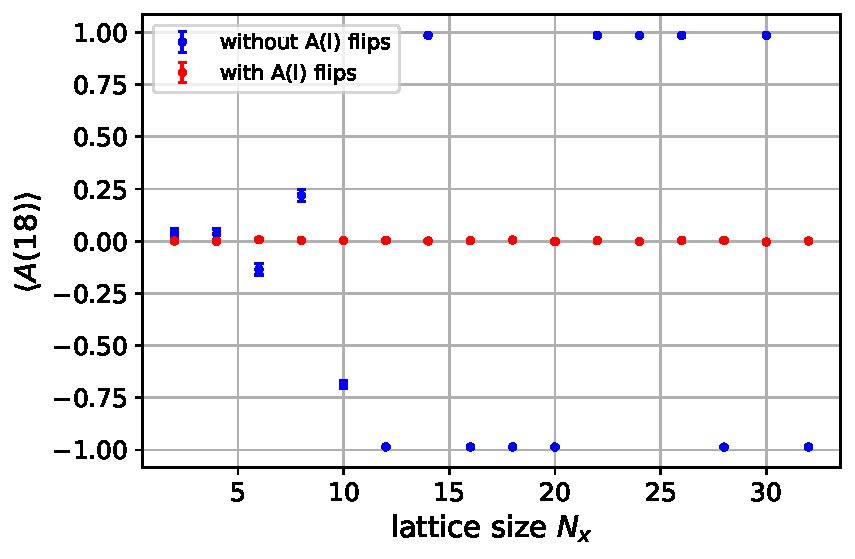
\includegraphics[width=\textwidth]{images/fix_subsystem_symmetry/expval(A(l)) vs N_x (l=18) with and without aflips.pdf}
    \end{subfigure}
    \caption{$\expval{A(l = 18)}$ both with and without alignment flips for different $N_x$.}
    \label{alignflipexpval}
\end{figure}
%%% FIG %%%
As proposed, the introduction of alignment flip proposals to the Metropolis algorithm makes the configuration space equally accessible in both positive and negative alignment regions. This leads to the $\expval{A(l)} \approx 0$ for all spatial lattice sizes, hence fixing the subsystem symmetry breaking. 
%%% FIG %%%
\begin{figure}[t!]
    \centering
    \begin{subfigure}[b]{0.5\textwidth}
        \centering
        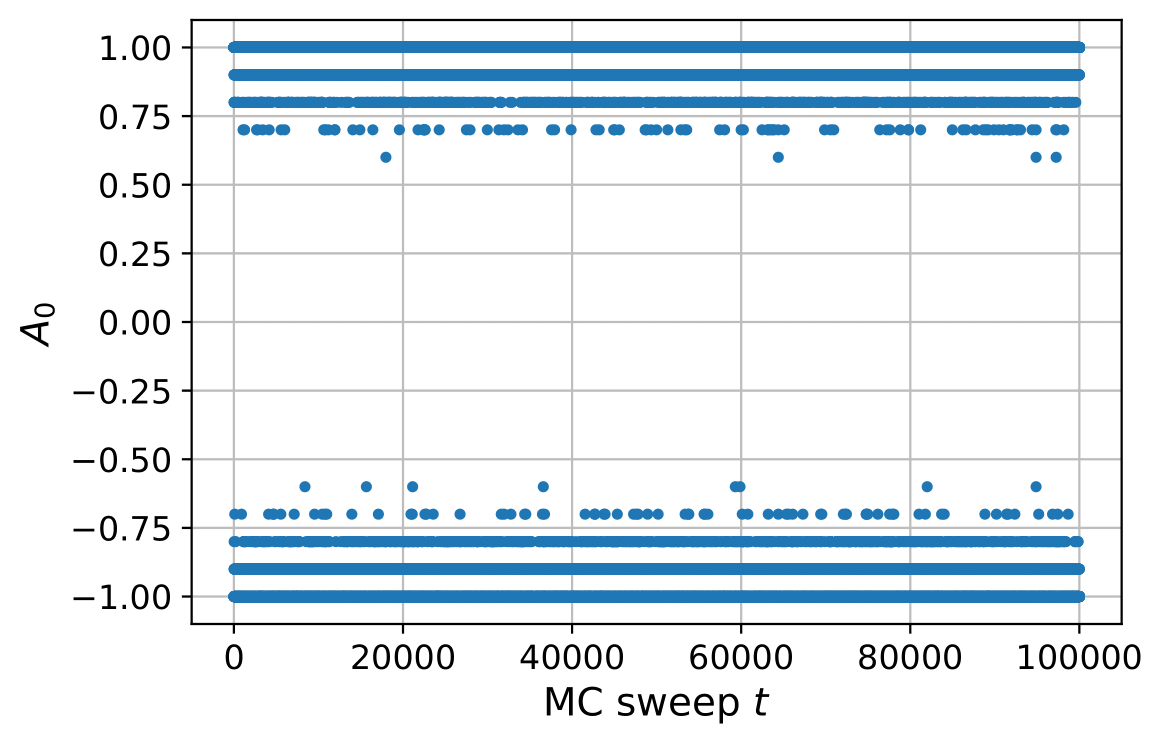
\includegraphics[width=\textwidth]{images/fix_subsystem_symmetry/measurement A(l) vs MC time (l=0).png}
        \caption{ $A(l)$ measurements vs MC time.}
    \end{subfigure}
    % \hspace{1em}  %\hfill
    \begin{subfigure}[b]{0.48\textwidth}
        \centering
        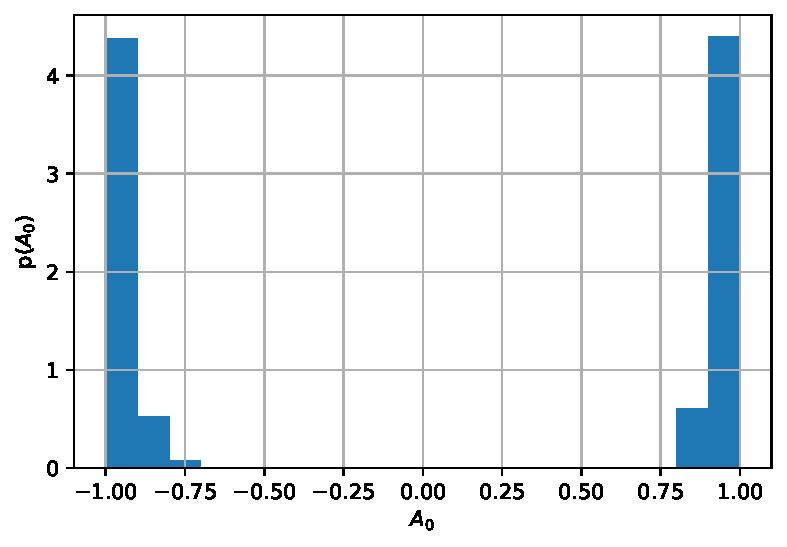
\includegraphics[width=\textwidth]{images/fix_subsystem_symmetry/measurement A(l) histogram (l=0).pdf}
        \caption{ $A(l)$ measurements histogram.}
    \end{subfigure}
    \caption{Configuration space exploring both $A(l)>0$ and $A(l)<0$ regions with alignment flip moves.}
    \label{alignflipmeasurements}
\end{figure}
%%% FIG %%%
% \FloatBarrier

This is also demonstrated in Fig.~\ref{alignflipmeasurements} where the Metropolis algorithm is shown to traverse both $A(l)>0$ and $A(l)<0$ regions of the configuration space. This verifies that ergodicity is indeed restored and the subsystem symmetry of the generalized classical Ising model is preserved.

\subsection{Autocorrelation function}
Since the alignment flips fixed the breaking of subsystem symmetry and freezing of the alignment values, we can now use the standard definition of the autocorrelation function 
\begin{equation}
    \text{Autocorr}[A_l] = \frac{1}{N-T} \sum_{k=0}^{N-T-1} \frac{(A_l(k) - \expval{A_l}) \cdot (A_l(k+T) - \expval{A_l}}{\expval{A_l(k)^2}}
\end{equation} 
where the average is taken over the first $N-T$ measurements, i.e.
\begin{equation}
    \langle{A_l(k)^2}\rangle = \frac{1}{N-T} \sum_{k=0}^{N-T-1} [A(k)]^2
\end{equation}
%%% FIG %%%
\begin{figure}[!htb]
    \centering
    \begin{subfigure}[b]{0.5\textwidth}
        \centering
        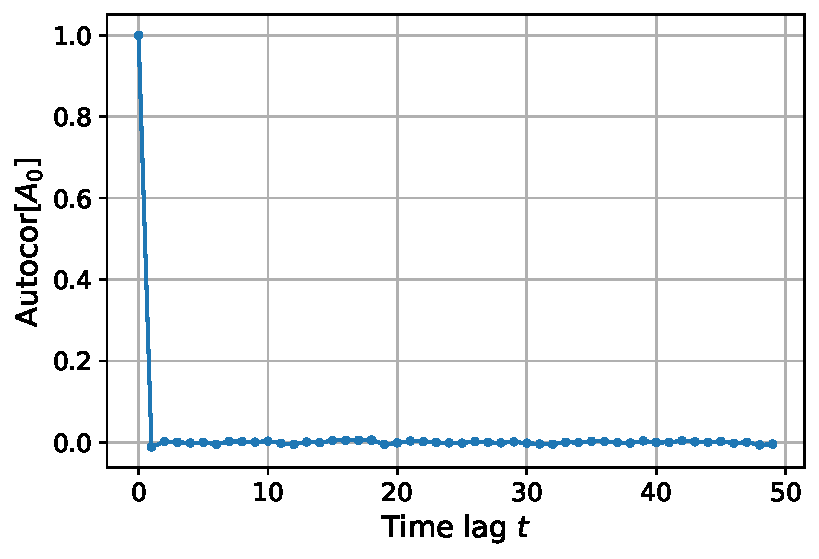
\includegraphics[width=\textwidth]{images/fix_subsystem_symmetry/Autocor[A(l)] (l=0).pdf}
    \end{subfigure}
    \caption{Autocorrelation function with alignment flips.}
    \label{alignflipautocorr}
\end{figure}
%%% FIG %%%
\FloatBarrier
Fig. \ref{alignflipautocorr} shows that the autocorrelation function drops extremely quickly when the simulation accesses all the allowed regions of the configuration space equally. For this particular simulation, the integrated autocorrelation time was calculated to be $\tau_\text{int} \approx 0.529$ implying that the alignment measurements $A(l)$ are highly uncorrelated in the Monte Carlo simulation.

This concludes our verification of the equilibration properties of our singlet Metropolis Monte Carlo algorithm. In the upcoming sections, we'll discuss methods to benchmark our quantum Monte Carlo implementation.
  
\section{Benchmarking quantum Monte Carlo}
Our previous results lead us to conclude that performing Metropolis Monte Carlo simulations by combining both spin flips and alignment flips keeps the subsystem symmetry of our system intact, and is a reliable way to perform calculations on the $(1+1)d$ generalized classical Ising model, equivalent to the $1d$ singlet Ising model.

However, the applicability of the quantum Monte Carlo calculations can only be verified when compared with analytical or a numerical calculations done directly on the quantum model. Remember that the strength of Monte Carlo simulations lies in the fact that it can work for higher lattice sizes without an exponential overhead in the computational cost. Therefore, the Metropolis Monte Carlo results are benchmarked against direct quantum calculations only for small lattice sizes. This should serve as a check for the pertinency of the quantum Monte Carlo simulations for the singlet Ising model.
\subsection{Singlet compatible operators}
Any operator $\hat{\mathcal{O}}$ defined on the singlet sector of the Hilbert space must satisfy 
\begin{equation}
    \hat{F} \: \hat{\mathcal{O}} \: \hat{F} \stackrel{!}{=} \hat{\mathcal{O}} \quad \implies [\hat{F}, \: \hat{\mathcal{O}}] \stackrel{!}{=} 0
    \label{operator}
\end{equation}
where $\hat{F} = \prod_i \hat{X}_i$ is the global flip operator as defined earlier in Eq. \ref{flipoperator}. The above constraint on the operators is a direct consequence of the singlet constraint on the singlet Hilbert space $\mathcal{H}_s$. Mathematically, this can be rephrased as follows - any operator $\mathcal{O}$ defined on $\mathcal{H}_s$ can be written in the outer product notation as 
\begin{equation}
    \hat{\mathcal{O}} = \sum_{i,\:j} c_{ij} \hat{P}\ket{\{\sigma\}}_i \bra{\{\sigma '\}}_j \hat{P}
\end{equation}
where $\hat{P} = (\mathds{1} + \hat{F})/2$ is the singlet projection operator. The action of $\hat{F}$ on $\hat{\mathcal{O}}$ from both sides gives   
\begin{equation}
    \hat{F} \: \hat{\mathcal{O}} \: \hat{F} = \sum_{ij} c_{ij} \: \underbrace{\hat{F}\hat{P}}_{ = \hat{P}} \: \ket{\{\sigma\}}_i \bra{\{\sigma '\}}_j \:\underbrace{\hat{P} \hat{F}}_{ = \hat{P}} = \sum_{i,j} c_{ij} \hat{P}\ket{\{\sigma\}}_i \bra{\{\sigma '\}}_j \hat{P} = \hat{\mathcal{O}}
\end{equation}
Thus any operator on the singlet sector $\hat{\mathcal{O}}: \mathcal{H}_s \to \mathcal{H}_s$ must satisfy  Eq.~\eqref{operator}. The two most elementary observables which satisfy this condition are $\hat{X}_i$ and $\hat{Z}_i \hat{Z}_j$.   Such singlet-compatible quantum operators can then be mapped to their corresponding classical analogs.  

\subsection{Mapping quantum operators to classical observables}
As always, the Hamiltonian with the singlet constraint is
\begin{equation}
    \hat{H} = - h \sum_i \hat{Z}_i \hat{Z}_j - J \sum_i \hat{X}_i, \qquad \prod_i X_i \stackrel{!}{=} \mathds{1}
\end{equation}
The quantum thermal expectation value of a singlet compatible operator $\hat{\mathcal{O}}$ can then be written as
\begin{align}
    \langle {\hat{\mathcal{O}}} \rangle  &= \frac{\Tr(e^{-\beta \hat{H}}\hat{\mathcal{O}})}{\Tr(e^{-\beta \hat{H}})} \nonumber \\
    &= \frac{1}{\mathcal{Z}} \sum_{\{\sigma_0 \}} \sum_{\mu_0, \lambda_0 \in \{\pm 1\}} \mel{\{\mu_0 \sigma _0\}}{e^{-\Delta \tau \hat{H}} e^{-\Delta \tau \hat{H}} \ldots e^{-\Delta \tau \hat{H}} \hat{\mathcal{O}}}{\{\lambda_0 \sigma _0\}}    
\end{align}
where we have again traced out the operators in the singlet basis, and sliced the $e^{-\beta \hat{H}}$ into $N_\tau$ smaller pieces. Using the cyclic property of trace, we can assert that $\hat{\mathcal{O}}$ does not have to be in the special position at the end of the operator product, therefore
\begin{align}
    \mathcal{Z} \cdot \langle {\hat{\mathcal{O}}} \rangle & = \frac{1}{N_\tau} \Bigg[ \sum_{\{\sigma_0 \}, \mu_0, \lambda_0} \mel{\{\mu_0 \sigma _0\}}{e^{-\Delta \tau \hat{H}} e^{-\Delta \tau \hat{H}} \ldots e^{-\Delta \tau \hat{H}} \hat{\mathcal{O}}}{\{\lambda_0 \sigma _0\}} \nonumber \\
    & + \sum_{\{\sigma_0 \}, \mu_0, \lambda_0} \mel{\{\mu_0 \sigma _0\}}{e^{-\Delta \tau \hat{H}} e^{-\Delta \tau \hat{H}} \ldots \hat{\mathcal{O}} e^{-\Delta \tau \hat{H}} }{\{\lambda_0 \sigma _0\}} \nonumber \\
    & + \sum_{\{\sigma_0 \}, \mu_0, \lambda_0} \mel{\{\mu_0 \sigma _0\}}{e^{-\Delta \tau \hat{H}} \ldots \hat{\mathcal{O}} e^{-\Delta \tau \hat{H}} e^{-\Delta \tau \hat{H}} }{\{\lambda_0 \sigma _0\}} \nonumber\\
    & \ldots  \: + \: \sum_{\{\sigma_0 \}, \mu_0, \lambda_0} \mel{\{\mu_0 \sigma _0\}}{\hat{\mathcal{O}} e^{-\Delta \tau \hat{H}} e^{-\Delta \tau \hat{H}} \ldots e^{-\Delta \tau \hat{H}}}{\{\lambda_0 \sigma _0\}} \Bigg]
\end{align}
Defining $\mu_{N_\tau} = \mu_0, \lambda _{N_\tau} = \lambda _0$, and $\{\sigma_{N_\tau}\} = \{\sigma_0\}$, and inserting the singlet identity 
\begin{equation}
    \mathds{1}_s = \sum_{\{\sigma_l \}, \mu_l, \lambda_l} \ket{\{\lambda_{l} \sigma_{l}\}}\bra{\{\mu_{l} \sigma_{l}\}}
\end{equation} 
for $l \in \{1, 2, 3 \ldots, N_\tau - 1\}$, we get the following expression
\begingroup
\allowdisplaybreaks
\begin{align}
    \mathcal{Z} \cdot \langle \hat{\mathcal{O}} \rangle = \qty(\prod_{l=0}^{N_\tau - 1} \sum_{\{\sigma_l \}, \mu_l, \lambda_l}) \frac{1}{N_\tau} \sum_{l_0 = 0}^{N_\tau - 1} \Bigg[\langle\{\mu_{l_0+1} & \sigma _{l_0+1}\}| {e^{-\Delta \tau \hat{H}} \hat{\mathcal{O}}}\ket{\{\lambda_{l_0} \sigma _{l_0}\}} \nonumber \\ 
    & \prod_{l \neq l_0} \mel{\{\mu_{l+1} \sigma _{l+1}\}}{e^{-\Delta \tau \hat{H}}}{\{\lambda_{l} \sigma _{l}\}} \Bigg] \qquad
    \label{generalop}
\end{align}
\endgroup
In the following subsections, we perform manipulations on Eq.~\eqref{generalop} for operators $\hat{X}_i$ and $\hat{Z}_i \hat{Z}_j$ to find the analogous classical observables.

\subsubsection{Classical analog of $\hat{Z}_i \hat{Z}_j$}
The classical analog of the $\hat{Z}_i \hat{Z}_j$ operator is now calculated by substituting $\hat{\mathcal{O}} =  \hat{Z}_i \hat{Z}_j$ in Eq.~\eqref{generalop}.
\begingroup
\allowdisplaybreaks
\begin{align}
    \mathcal{Z} \cdot \langle {\hat{Z}_i \hat{Z}_j} \rangle &= \qty(\prod_{l=0}^{N_\tau - 1} \sum_{\{\sigma_l \}, \mu_l, \lambda_l}) \frac{1}{N_\tau} \sum_{l_0 = 0}^{N_\tau - 1} \Bigg[\langle\{\mu_{l_0+1} \sigma _{l_0+1}\}|{e^{-\Delta \tau \hat{H}}{\hat{Z}_i \hat{Z}_j}}|{\{\lambda_{l_0} \sigma _{l_0}\}} \rangle \qquad \qquad \nonumber\\
    &\qquad \qquad \qquad \qquad \qquad \qquad \qquad \qquad \prod_{l \neq l_0} \mel{\{\mu_{l+1} \sigma _{l+1}\}}{e^{-\Delta \tau \hat{H}}}{\{\lambda_{l} \sigma _{l}\}} \Bigg] \nonumber \\
    & =  \qty(\prod_{l=0}^{N_\tau - 1} \sum_{\{\sigma_l \}, \mu_l, \lambda_l}) \frac{1}{N_\tau} \sum_{l_0 = 0}^{N_\tau - 1} \Bigg[\mel{\{\mu_{l_0+1} \sigma _{l_0+1}\}}{e^{-\Delta \tau \hat{H}}}{\{\lambda_{l_0} \sigma _{l_0}\}} (\lambda_{l_0} \sigma^i_{l_0})(\lambda_{l_0} \sigma^j_{l_0}) \qquad \qquad \nonumber \\ 
    & \qquad \qquad \qquad \qquad \qquad \qquad \qquad \qquad \prod_{l \neq l_0} \mel{\{\mu_{l+1} \sigma _{l+1}\}}{e^{-\Delta \tau \hat{H}}}{\{\lambda_{l} \sigma _{l}\}}\Bigg] \nonumber \\ 
    & = \qty(\prod_{l=0}^{N_\tau - 1} \sum_{\{\sigma_l \}, \mu_l, \lambda_l}) \qty(\frac{1}{N_\tau} \sum_{l_0 = 0}^{N_\tau - 1} \sigma^i_{l_0} \sigma^j_{l_0}) \qty[\prod_{l = 0}^{N_\tau - 1} \mel{\{\mu_{l+1} \sigma _{l+1}\}}{e^{-\Delta \tau \hat{H}}}{\{\lambda_{l} \sigma _{l}\}}]
\end{align}
\endgroup
where we have used the shorthand notation $\sigma_{l}(i) \equiv \sigma^{i}_l$. After performing a few manipulations on the $\prod_l$ product of terms, and performing a sum over $\mu_l, \lambda_l \in \{\pm 1\}$, we obtain a similar discrete path integral as we do for the quantum to classical correspondence of the partition function, over the standard spin basis $\{\sigma_l\}$
\begin{equation}
    \langle {\hat{Z}_i \hat{Z}_j} \rangle = \frac{1}{\mathcal{Z}} \qty(\prod_{l=0}^{N_\tau - 1} \sum_{\{\sigma_l \}}) \qty(\frac{1}{N_\tau} \sum_{l_0 = 0}^{N_\tau - 1} \sigma^i_{l_0} \sigma^j_{l_0}) e^{-S[\sigma]}
\end{equation}
where $S[\sigma]$ is the effective classical action of the generalized Ising model Eq.~\eqref{classicalaction}. Therefore, the classical observable corresponding to quantum operator $\hat{Z}_i \hat{Z}_j$ is given by
\begin{equation}
    O_{Z_i Z_j} = \frac{1}{N_\tau} \sum_{l = 0}^{N_\tau - 1} \sigma^i_{l} \sigma^j_{l}
    \label{classicalzizj}
\end{equation}~\\
\subsubsection{Classical analog of $\hat{X}_i$}
Following a similar procedure as above, we also calculate the classical observable corresponding to $\hat{X}_i$, although the calculation isn't as straightforward here

\begingroup
\allowdisplaybreaks
\begin{align}
    \mathcal{Z} \cdot \langle {\hat{X}_i} \rangle
    = \qty(\prod_{l=0}^{N_\tau - 1} \sum_{\{\sigma_l \}, \mu_l, \lambda_l}) \frac{1}{N_\tau} \sum_{l_0 = 0}^{N_\tau - 1} \Bigg[\langle\{\mu_{l_0+1}& \sigma _{l_0+1}\}|{e^{-\Delta \tau \hat{H}} \hat{X}_i}|{\{\lambda_{l_0} \sigma _{l_0}\}}\rangle \qquad \nonumber \\ 
    & \prod_{l \neq l_0} \mel{\{\mu_{l+1} \sigma _{l+1}\}}{e^{-\Delta \tau \hat{H}}}{\{\lambda_{l} \sigma _{l}\}} \Bigg]
    \label{operator_x_i}
\end{align}
\endgroup
Let us first analyze the matrix element containing the $\hat{X}_i$
\begin{equation}
    \mel{\{\mu_{l_0+1} \sigma _{l_0+1}\}}{e^{-\Delta \tau \hat{H}} \hat{X}_i}{\{\lambda_{l_0} \sigma _{l_0}\}} \approx \mel{\{\mu_{l_0+1} \sigma _{l_0+1}\}}{e^{-\Delta \tau \hat{H}_I} e^{-\Delta \tau \hat{H}_T} \hat{X}_i}{\{\lambda_{l_0} \sigma _{l_0}\}}
    \label{1.6.13}
\end{equation}
The above approximation is valid in the limit $\Delta \tau \to 0$ and $N_\tau \to \infty$. If we make the Ising interaction term $\hat{H}_I$ act on the bra at the left, we get
\begin{align}
    \text{Eq.~\eqref{1.6.13} }& = \mel{\{\mu_{l_0+1} \sigma _{l_0+1}\}}{e^{-\Delta \tau \hat{H}_T} \hat{X}_i}{\{\lambda_{l_0} \sigma _{l_0}\}} e^{-\Delta \tau \hat{H}_I(\{\mu_{l_0+1} \sigma_{l_0+1}\})} \nonumber && \\
    & = \mel{\{\mu_{l_0+1} \sigma _{l_0+1}\}}{e^{-\Delta \tau \hat{H}_T} \hat{X}_i}{\{\lambda_{l_0} \sigma _{l_0}\}} e^{-\Delta \tau \hat{H}_I(\{\sigma_{l_0+1}\})} \nonumber && \\
    & = \mel{\{\mu_{l_0+1} \sigma _{l_0+1}\}}{e^{-\Delta \tau \hat{H}_T} \hat{X}_i}{\{\lambda_{l_0} \sigma _{l_0}\}} e^{-\Delta \tau \hat{H}_I(\{\sigma_{l_0}\})}
\end{align}
Ignoring the Ising term for now, we can write $\mel{\{\mu_{l_0+1} \sigma _{l_0+1}\}}{e^{-\Delta \tau \hat{H}_T} \hat{X}_i}{\{\lambda_{l_0} \sigma _{l_0}\}}$ term as follows 
\begin{align}
    \mel{\{\mu_{l_0+1} \sigma _{l_0+1}\}}{e^{-\Delta \tau \hat{H}_T} \hat{X}_i}{\{\lambda_{l_0} \sigma _{l_0}\}} = \mel{\{\mu_{l_0+1} \sigma _{l_0+1}\}}{e^{\Delta \tau \sum_j \hat{X}_j} \hat{X}_i}{\{\lambda_{l_0} \sigma _{l_0}\}} \nonumber \\
    = \mel{\mu_{l_0+1} \sigma^i_{l_0+1}}{e^{\Delta \tau \hat{X}_i} \hat{X}_i}{\lambda_{l_0} \sigma^i_{l_0}} \prod_{j \neq i} \mel{\mu_{l_0+1} \sigma^j_{l_0+1}}{e^{\Delta \tau \hat{X}_j}}{\lambda_{l_0} \sigma^j_{l_0}}  
    \label{matrixproducts}
\end{align} 
The above outer products can be written in a simpler fashion,
\begin{flalign}
    & e^{\Delta \tau J \hat{X}_j} = \cosh(\Delta \tau J) \mathds{1} + \sinh(\Delta \tau J) \hat{X}_j \nonumber \\
    & e^{\Delta \tau J \hat{X}_i} \hat{X}_i = \sinh(\Delta \tau J) \mathds{1} + \cosh(\Delta \tau J) \hat{X}_i 
    \end{flalign}
Therefore, when we evaluate the matrix products Eq.~\eqref{matrixproducts}, we get 
\begin{flalign}
    & \mel{\mu_{l_0+1} \sigma^j_{l_0+1}}{e^{\Delta \tau \hat{X}_j}}{\lambda_{l_0} \sigma^j_{l_0}} = A e^{+K \mu_{l_0 + 1} \lambda_{l_0} \sigma^j_{l_0+1} \sigma^j_{l_0}} \nonumber \\
    & \mel{\mu_{l_0+1} \sigma^i_{l_0+1}}{e^{\Delta \tau \hat{X}_i} \hat{X}_i}{\lambda_{l_0} \sigma^i_{l_0}} = A e^{- K \mu_{l_0 + 1} \lambda_{l_0} \sigma^j_{l_0+1} \sigma^j_{l_0}}
    \label{1.6.19}
\end{flalign}
where $A = \sqrt{\frac{1}{2} \sinh(2J \Delta \tau)}$ and $K = \frac{1}{2} \ln\tanh(J \Delta \tau)$. It is the $\hat{X}$ operator that flips the sign of the factor in the exponential when $j = i, \: l = l_0$. This is key difference in the calculations when compared to $\mathcal{Z}$. Combining Eqs.~\eqref{matrixproducts} and~\eqref{1.6.19}, the matrix product term for the layer $l_0$ (with $\hat{X}_i$) can be simply written as

\begin{gather}
    \mel{\{\mu_{l_0+1} \sigma _{l_0+1}\}}{e^{-\Delta \tau \hat{H}_T} \hat{X}_i}{\{\lambda_{l_0} \sigma _{l_0}\}} = A^{N_x} e^{-K(\mu_{l_0 + 1} \lambda_{l_0})\sigma^i_{l_0+1} \sigma^i_{l_0}} \prod_{j \neq i} e^{+ K(\mu_{l_0 + 1} \lambda_{l_0})\sigma^j_{l_0+1} \sigma^j_{l_0}} \nonumber \\
    = A^{N_x} \exp\qty(-2K(\mu_{l_0 + 1} \lambda_{l_0})\sigma^i_{l_0+1} \sigma^i_{l_0}) \exp\qty( K(\mu_{l_0 + 1} \lambda_{l_0}) \sum_{j = 0}^{N_x-1} \sigma^j_{l_0+1} \sigma^j_{l_0}) 
    \label{part a}
\end{gather}
For the matrix product associated to all the other layers $l \neq l_0$ (without $\hat{X}_i$), the calculation proceeds similarly and we get
\begin{equation}
    \mel{\{\mu_{l+1} \sigma _{l+1}\}}{e^{-\Delta \tau \hat{H}_T}}{\{\lambda_{l} \sigma _{l}\}} = A^{N_x}
    \exp\qty(K(\mu_{l + 1} \lambda_{l}) \sum_{j = 0}^{N_x-1} \sigma^j_{l+1} \sigma^j_{l})
    \label{part b}
\end{equation}
Combining the matrix element expressions from both Eqs.~\eqref{part a} and \eqref{part b}, we can write the expectation value sum as follows (ignoring the proportionality constants)
\begin{align}
    \mathcal{Z} \cdot \langle \hat{X}_i \rangle = \qty(\prod_{l=0}^{N_\tau - 1} \sum_{\{\sigma_l \}, \mu_l, \lambda_l}) \Bigg(\frac{1}{N_\tau} \sum_{l_0 = 0}^{N_\tau - 1} & e^{-2K \mu_{l_0 + 1} \lambda_{l_0} \sigma^{i}_{l_0} \sigma^{i}_{l_0 + 1}}\Bigg)  \nonumber \\ 
    & \prod_{l = 0}^{N_\tau - 1} e^{K \mu_{l+1} \lambda_l \sum_j \sigma^j_{l+1} \sigma ^j_l + h \Delta \tau \sum_j \sigma^j_l \sigma^{j+1}_l}
\end{align}
Since the expectation value $\langle \hat{X}_i \rangle$ only depends on the product $\mu_{l+1}\lambda_l$, and we are summing over $\lambda_l, \mu_{l+1} \in \{\pm 1\}$, we can replace it by just $\mu_l$ with the values lying $\in \{\pm 1\}$.
% \hspace*{-1.7cm}
\begin{align}
    & =  \qty(\prod_{l=0}^{N_\tau - 1} \sum_{\{\sigma_l \}}) \frac{1}{N_\tau} \sum_{l_0 = 0}^{N_\tau - 1} \Bigg[\qty(\sum_{\mu_{l_0}} e^{K \mu_{l_0+1} \sum_j \sigma^j_{l_0+1} \sigma^j_{l_0} - 2K \mu_{l_0 + 1}  \sigma^{i}_{l_0} \sigma^{i}_{l_0 + 1}}) e^{ h \Delta \tau  \sum_j \sigma^j_{l_0} \sigma^{j+1}_{l_0}} \nonumber \\
    & \qquad\qquad\qquad\qquad\qquad\qquad\qquad\qquad\prod_{l \neq l_0} \sum_{\mu_{l}} e^{K \mu_{l+1} \sum_j \sigma^j_{l+1} \sigma ^j_l + h \Delta \tau  \sum_j \sigma^j_l \sigma^{j+1}_l} \Bigg] \nonumber \\
    & = \qty(\prod_{l=0}^{N_\tau - 1} \sum_{\{\sigma_l \}}) \frac{1}{N_\tau} \sum_{l_0 = 0}^{N_\tau - 1} \Bigg[ \cosh\qty(K \sum_j \sigma^j_{l_0+1} \sigma^j_{l_0} - 2K \sigma^{i}_{l_0} \sigma^{i}_{l_0 + 1}) e^{ h \Delta \tau  \sum_j \sigma^j_{l_0} \sigma^{j+1}_{l_0}} \nonumber \\
    &   \qquad\qquad\qquad\qquad\qquad\qquad\qquad\qquad\prod_{l \neq l_0} \cosh\qty(K \sum_j \sigma^j_{l+1} \sigma ^j_l) e^{h \Delta \tau  \sum_j \sigma^j_l \sigma^{j+1}_l} \Bigg] 
    \label{almostfinal}
\end{align}
Finally, we can expand the $\cosh(x-y)$ term in Eq. \eqref{almostfinal}, take out $\cosh(K \sum_j \sigma^j_{l_0+1} \sigma^j_{l_0})$ $e^{ h \Delta \tau  \sum_j \sigma^j_{l_0} \sigma^{j+1}_{l_0}}$ as a common factor, and restore the $\displaystyle \prod_{l \neq l_0}$ to $\displaystyle\prod_{l = 0}^{N_\tau - 1}$. The product then converts into the usual Boltzmann factor $e^{-S[\sigma]}$ leaving behind the classical observable,

\begin{align}
    \langle \hat{X}_i \rangle = \frac{1}{\mathcal{Z}} \Bigg(\prod_{l=0}^{N_\tau - 1}& \sum_{\{\sigma_l \}}\Bigg) \frac{1}{N_\tau} \sum_{l_0 = 0}^{N_\tau - 1} \Bigg(\cosh\big(2K \sigma^{i}_{l_0} \sigma^{i}_{l_0 + 1}\big) \nonumber \\
    &-\tanh\big(K \sum_j \sigma^j_{l_0+1} \sigma^j_{l_0}\big) \sinh\qty(2K \sigma^{i}_{l_0} \sigma^{i}_{l_0 + 1}) \Bigg)e^{-S[\sigma]}
\end{align}
Thus, the extracted classical observable corresponding to the quantum operator $\hat{X}_i$ as
\begin{equation}
        O_{{X}_i} = \frac{1}{N_\tau} \sum_{l=0}^{N_\tau -1} \qty[\cosh(2K\sigma^{i}_{l} \sigma^{i}_{l + 1}) - \tanh\qty(K \sum_{j=0}^{N_x-1} \sigma^j_{l+1} \sigma^j_{l}) \sinh\qty(2K \sigma^{i}_{l} \sigma^{i}_{l + 1})]
     \label{classicalxi_1}
\end{equation} 
Using a few trigonometric identities, it can be written compactly as 
\begin{equation}
        O_{{X}_i} = \frac{1}{N_\tau} \sum_{l=0}^{N_\tau -1} \qty[\frac{\cosh\qty(2K\sigma^{i}_{l} \sigma^{i}_{l + 1} - K \sum_{j=0}^{N_x-1} \sigma^j_{l+1} \sigma^j_{l})}{\cosh\qty(K \sum_{j=0}^{N_x-1} \sigma^j_{l+1} \sigma^j_{l})}]
    \label{classicalxi_2}
\end{equation}
The central idea surrounding the benchmarking of the quantum Monte Carlo simulations involves comparing the Monte Carlo averages of classical observables $O_{X_i}$ and $O_{Z_i Z_j}$ against the quantum expectation values of quantum operators $\hat{X}_i$ and $\hat{Z}_i \hat{Z}_j$. This is discussed in the following sections.   
% \VBS{The indices on the two sides do not seem to match. Should it be $\cosh{(2K \sigma^i_l \sigma^i_{l+1})} $...I have not yet fully checked things, but something seems not quite clean.}

% \KV{Extremely sorry for the goof up. You are right, I made an error in the indices with the $2K$ term. It should have had the $i$ index instead of $j$. I have fixed it now.}

\section{The two site problem}
The two site problem for the singlet Ising model serves as the simplest non-trivial problem. The two site quantum chain with $N_x = 2$ displays the simplest quantum features of the problem while also being analytically tractable. As the most elementary exercise, it is vital to verify that analytical results for the quantum expectation values of $\hat{X}_i$ and $\hat{Z}_i \hat{Z}_j$ match with the Monte Carlo averages performed for the classical observables $O_{X_i}$ and $O_{Z_i Z_j}$.

\subsection{Quantum expectation values}
For two spin sites, the Hilbert space can be defined to be spanned by the singlet basis
\begin{equation}
    \mathcal{H}_s = \text{span} \left\{\frac{\ket{\uparrow \uparrow} + \ket{\downarrow\downarrow}}{\sqrt{2}}, \frac{\ket{\uparrow\downarrow} + \ket{\downarrow\uparrow}}{\sqrt{2}} \right\}
\end{equation}
The above states are labelled as
\begin{equation} 
    \ket{a} = \frac{\ket{\uparrow \uparrow} + \ket{\downarrow\downarrow}}{\sqrt{2}}, \qquad \ket{b} = \frac{\ket{\uparrow\downarrow} + \ket{\downarrow\uparrow}}{\sqrt{2}}
\end{equation}
The expression for the expectation value of an operator is given by 
\begin{equation}
    \langle{\hat{O}}\rangle = \Tr(e^{-\beta \hat{H}} \hat{O}) = \frac{e^{-\beta E_0}\mel{w_0}{\hat{O}}{w_0} + e^{-\beta E_1}\mel{w_1}{\hat{O}}{w_1}}{e^{-\beta  E_0} + e^{-\beta E_1}}
\end{equation}
where we have evaluated the trace in the yet-unknown energy eigenbasis. The energy eigenvalues $E_i$ and the eigenvectors $\ket{w_i}$ can be calculated by diagonalizing the Hamiltonian in the singlet basis representation.
\begin{equation}
    H := \left(\begin{array}{cc}
    \mel{a}{\hat{H}}{a} & \mel{a}{\hat{H}}{b} \\ 
    \mel{b}{\hat{H}}{a} & \mel{a}{\hat{H}}{b}
    \end{array}\right)
\end{equation}
For $N_x = 2$, the quantum Hamiltonian with periodic boundary conditions simplifies to
\begin{equation}
    \hat{H} = - 2h \hat{Z}_0 \hat{Z}_1 - J(\hat{X}_0 + \hat{X}_1)
\end{equation}
and after a bit of algebra, the matrix representation in the singlet basis comes out to be
\begin{equation}
    H:= \left(\begin{array}{cc}
    -2h & -2J \\ 
    -2J & 2h
    \end{array}\right)
\end{equation}
Thus, the energy eigenvalues obtained on solving the secular equation gives the following
\begin{equation}
    \lambda_\pm = \pm 2 \sqrt{h^2 + J^2}
\end{equation}
Let us define 
\begin{equation}
    h = B \cos \theta, \qquad \qquad J = B \sin \theta
\end{equation}
Then $\lambda_\pm = \pm 2B$, and the $\hat{H}$ matrix becomes
\begin{equation}
    H := 2B \left(\begin{array}{cc}
    -\cos \theta  & -\sin \theta  \\ 
    -\sin \theta  & \cos \theta 
    \end{array}\right)
\end{equation}
To find the eigenvectors, we claim that one of them is given by 
\begin{equation}
    \ket{w_0} = u \ket{a} + v \ket{b}
\end{equation}
This implies that the other eigenvector must be of the form
\begin{equation}
    \ket{w_1} = -v \ket{a} + u \ket{b}
\end{equation}
with $u$ and $v$ $\in \mathbb{R}$ to satisfy the orthonormality relations. 

For the eigenvector $\ket{w_0}$  with the eigenvalue $E_0 = -2B$, the matrix equation can be written as follows
\begingroup
\allowdisplaybreaks
\begin{align}
    & 2B \left(\begin{array}{cc}
    -\cos \theta  & -\sin \theta  \\ 
    -\sin \theta  & \cos \theta 
    \end{array}\right) = -2B 
    \left(\begin{array}{c}
    u \\ 
    v
    \end{array}\right) \nonumber\\
    & 2B \left(\begin{array}{cc}
    -\cos \theta +1 & -\sin \theta  \\ 
    - \sin \theta  & \cos \theta + 1
    \end{array}\right)
    \left(\begin{array}{c}
    u \\ 
    v
    \end{array}\right) = 
    \left(\begin{array}{c}
    0 \\ 
    0
    \end{array}\right) \nonumber\\ 
    & 2B \left(\begin{array}{cc}
    2 \sin^2(\theta/2) & -2\sin(\theta /2) \cos(\theta /2) \\ 
    -2 \sin(\theta /2) \cos(\theta /2) & 2 \cos^2(\theta /2)
    \end{array}\right) 
    \left(\begin{array}{c}
    u \\ 
    v
    \end{array}\right) = 
    \left(\begin{array}{c}
    0 \\ 
    0
    \end{array}\right)
\end{align}
\endgroup
Solving for $u$ and $v$, we obtain the relation 
\begin{gather}
    \sin (\theta /2) u = \cos (\theta /2) v \nonumber \\
    \implies u = \cos(\theta /2), \qquad v = \sin (\theta /2) \qquad
\end{gather}
Let us now calculate the matrix elements $\mel{w_i}{\hat{O}}{w_i}$ for $\hat{O} = \hat{X}_i$, which are used in the evaluation of the thermal expectation value of $\hat{X}_i$.
\begingroup
\allowdisplaybreaks
\begin{align}
    \mel{w_0}{\hat{X}_0}{w_0} & = (\bra{a} u + \bra{b} v) \hat{X}_i (u \ket{a} + v \ket{b}) \nonumber\\
    & = u^2 \bra{a}\underbrace{{\hat{X}_0}\ket{a}}_{\ket{b}} +  uv \bra{a}\underbrace{{\hat{X}_0}\ket{b}}_{\ket{a}} + uv \bra{b}\underbrace{{\hat{X}_0}\ket{a}}_{\ket{b}} + v^2 \bra{b}\underbrace{{\hat{X}_0}\ket{b}}_{\ket{a}} \nonumber\\ 
    & = u^2 \braket{a}{b} + uv \braket{a}{a} + uv \braket{b}{b} + v^2\braket{b}{a} \nonumber\\
    & = 2uv
\end{align}
\endgroup
\begingroup
\allowdisplaybreaks
\begin{align}
    \mel{w_1}{\hat{X}_0}{w_1} & = (-\bra{a}v + \bra{b} u) \hat{X}_i (-v \ket{a} + u \ket{b}) \nonumber\\
    & = v^2 \bra{a}\underbrace{{\hat{X}_0}\ket{a}}_{\ket{b}} -  uv \bra{a}\underbrace{{\hat{X}_0}\ket{b}}_{\ket{a}} - uv \bra{b}\underbrace{{\hat{X}_0}\ket{a}}_{\ket{b}} + u^2 \bra{b}\underbrace{{\hat{X}_0}\ket{b}}_{\ket{a}} \nonumber\\ 
    & = v^2 \braket{a}{b} - uv \braket{a}{a} - uv \braket{b}{b} + u^2\braket{b}{a} \nonumber\\
    & = -2uv
\end{align}
\endgroup
The calculation is exactly similar for $\hat{X}_1$. The expectation value for $\hat{X}$  then evaluates to 
\begin{align}
    \langle \hat{X} \rangle & = 2uv \qty(\frac{e^{2\beta B} - e^{-2\beta B}}{e^{2\beta B} + e^{-2\beta B}}) = 2uv \tanh (2\beta B) \nonumber \\ 
    & \implies \langle{\hat{X}}\rangle = \frac{J}{B} \tanh(2\beta B)
    \label{X-hat_expval}
\end{align}
The calculation for $\hat{Z}_0 \hat{Z}_1$ is analogous and the matrix elements are evaluated as follows
\begin{align}
    \mel{w_0}{\hat{Z}_0 \hat{Z}_1}{w_0} & = (\bra{a} u + \bra{b} v) \hat{Z}_0 \hat{Z}_1 (u \ket{a} + v \ket{b}) \nonumber\\
    & = u^2 \bra{a}\underbrace{{\hat{Z}_0 \hat{Z}_1}\ket{a}}_{\ket{a}} +  uv \bra{a}\underbrace{{\hat{Z}_0 \hat{Z}_1}\ket{b}}_{-\ket{b}} + uv \bra{b}\underbrace{{\hat{Z}_0 \hat{Z}_1}\ket{a}}_{\ket{a}} + v^2 \bra{b}\underbrace{{\hat{Z}_0 \hat{Z}_1}\ket{b}}_{-\ket{b}} \nonumber\\ 
    & = u^2 \braket{a}{a} - uv \braket{a}{b} + uv \braket{b}{a} - v^2\braket{b}{b} \nonumber\\
    & = u^2 - v^2
\end{align}
\begin{align}
    \mel{w_1}{\hat{Z}_0 \hat{Z}_1}{w_1} & = (-\bra{a}v + \bra{b} u) \hat{Z}_0 \hat{Z}_1 (-v \ket{a} + u \ket{b}) \nonumber\\
    & = v^2 \bra{a}\underbrace{{\hat{Z}_0 \hat{Z}_1}\ket{a}}_{\ket{a}} -  uv \bra{a}\underbrace{{\hat{Z}_0 \hat{Z}_1}\ket{b}}_{-\ket{b}} - uv \bra{b}\underbrace{{\hat{Z}_0 \hat{Z}_1}\ket{a}}_{\ket{a}} + u^2 \bra{b}\underbrace{{\hat{Z}_0 \hat{Z}_1}\ket{b}}_{-\ket{b}} \nonumber\\ 
    & = v^2 \braket{a}{a} - uv \braket{a}{b} + uv \braket{b}{a} - u^2\braket{b}{b} \nonumber\\
    & = -(u^2 - v^2)
\end{align}
Therefore, the expectation value of $\hat{Z}_0 \hat{Z}_1$ evaluates to 
\begin{align}
    \langle \hat{Z}_0 \hat{Z}_1 \rangle & = (u^2-v^2) \qty(\frac{e^{2\beta B} - e^{-2\beta B}}{e^{2\beta B} + e^{-2\beta B}}) = (u^2-v^2) \tanh (2\beta B) \nonumber \\ 
    & \implies \langle{\hat{Z}_0 \hat{Z}_1}\rangle = \frac{h}{B} \tanh(2\beta B)
    \label{ZZ-hat_expval}
\end{align}

\subsection{Monte Carlo averages}
The effective classical action arising out of quantum to classical correspondence looks much simpler for $N_x=2$   
\begin{equation}
    S = - 2h \Delta \tau \sum_{l=1}^{N_\tau} \sigma^{0}_l \sigma^{1}_{l} - \sum_{l=1}^{N_\tau} \ln \cosh \qty[K \qty(\sigma^0_l \sigma^0_{l+1} + \sigma^1_l \sigma^1_{l+1})] 
\end{equation}
Thus, for a spin flip $\sigma^{i_0}_{l_0} \to - \sigma^{i_0}_{l_0}$, we can decompose the change in action as 
\[
    \Delta S_x = 4 h \Delta \tau \sigma^{0}_{l_0} \sigma^{1}_{l_0}  
\]
\[
    \Delta S_\tau = \ln \qty[ \frac{\cosh\qty[K(\sigma^{0}_{l} \sigma^{0}_{l+1} + \sigma^{1}_{l} \sigma^{1}_{l+1} )] \cdot \cosh\qty[K(\sigma^{0}_{l} \sigma^{0}_{l-1} + \sigma^{1}_{l} \sigma^{1}_{l-1} )] }{\cosh\qty[K(\sigma^{0}_{l} \sigma^{0}_{l+1} - \sigma^{1}_{l} \sigma^{1}_{l+1} )] \cdot \cosh\qty[K(\sigma^{0}_{l} \sigma^{0}_{l-1} - \sigma^{1}_{l} \sigma^{1}_{l-1} )]}  ]
\]

\begin{equation}
    \Delta S = \Delta S_x + \Delta S_\tau 
\end{equation}
As before, the relevant operators are the mappings of $\hat{X}_i$ and $\hat{Z}_0 \hat{Z}_1$, i.e., the classical observables $O_{X}$ and $O_{Z_0 Z_1}$ respectively.
\begin{equation}
    O_{Z_0 Z_1} = \frac{1}{N_\tau} \sum_{l=0}^{N_\tau - 1} \sigma^0_l \sigma^1_l
\end{equation}
\begin{equation}
    O_X = O_{X_0} = O_{X_1} = \frac{1}{N_\tau} \sum_{l=0}^{N_\tau -1} \Bigg[\frac{\cosh\big( K \sigma^0_l \sigma^0_{l+1} - K \sigma^1_l \sigma^1_{l+1} \big)}{\cosh\big( K \sigma^0_l \sigma^0_{l+1} + K \sigma^1_l \sigma^1_{l+1} \big)}  \Bigg]
\end{equation}
Finally, we can then use our modified Metropolis Monte Carlo algorithm with spin flips and alignment flips, defined with an acceptance probability of $\text{min} (1, e^{-\Delta S})$. These Monte Carlo averages of $O_X$ and $O_{Z_0 Z_1}$ are then compared against the analytical results for $\langle \hat{X} \rangle$ and $\langle \hat{Z}_0 \hat{Z}_1\rangle$.

\subsection{Comparing Monte Carlo against analytical results}

We perform the Monte Carlo simulation for $\beta = N_\tau = 50$, keeping $\Delta \tau = 1$ and alignment flip fraction $f = \texttt{1.0}$. However, care needs to be taken while choosing the values of $J$ (consequently $K$) and $h$ (consequently $Y$). Since the model only depends on the ratio $J/h$, we have the freedom of choosing the value of the parameters as large or as small as we want. To explore the system near $J/h = 1$, we have to adjust the parameter values accordingly. If $Y$ is too small, then the values of $K$ near $J/h = 1$ are too large and that results in a low \textit{acceptance rate} and high \textit{trotter error}. The values of $K$ near $J/h = 1$ are small if $h$ is large, but it again results in the same problem. Moreover, disproportionate orders of magnitude of $K$ and $Y$ can lead to spin freezing along one of the directions.

Therefore, we require an optimum range of values for parameters $K$ and $Y$ to explore the system near the $J/h = 1$ point so as to minimize the \textit{trotter error} and maximize the \textit{acceptance rate}. Therefore, we choose $Y = \texttt{0.05}$ and vary $K$. The $J/h = 1$ then translates $K_* = 1.498$, so we choose values of $K$ so as to explore the system near this value.    
%%% FIG %%%
\begin{figure}[!htb]
    \centering
    \begin{subfigure}[b]{0.49\textwidth}
        \centering
        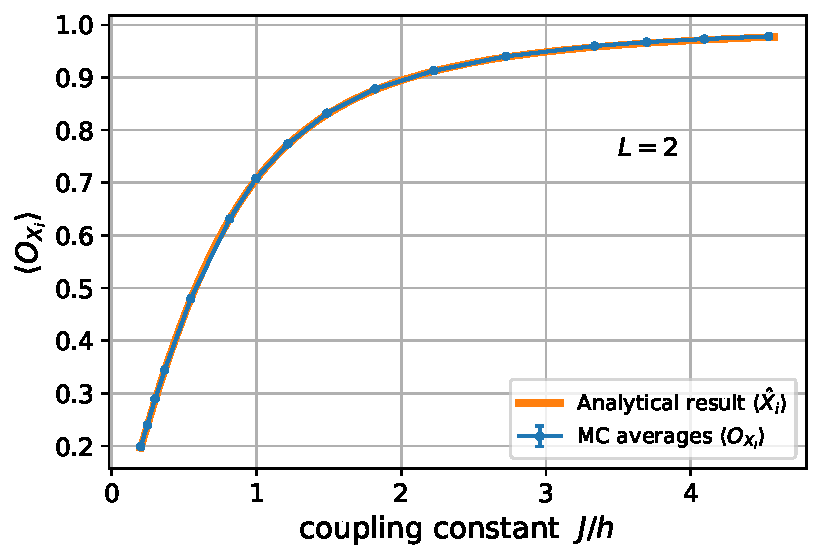
\includegraphics[width=\textwidth]{images/2_site/O_X.pdf}
        \caption{Monte Carlo average $\expval{O_X}$ vs. $J/h$.}
        \label{expval_O_X_vs_J/h_2}
    \end{subfigure}
    \begin{subfigure}[b]{0.49\textwidth}  %keep total sum <1 to show in same line
        \centering
        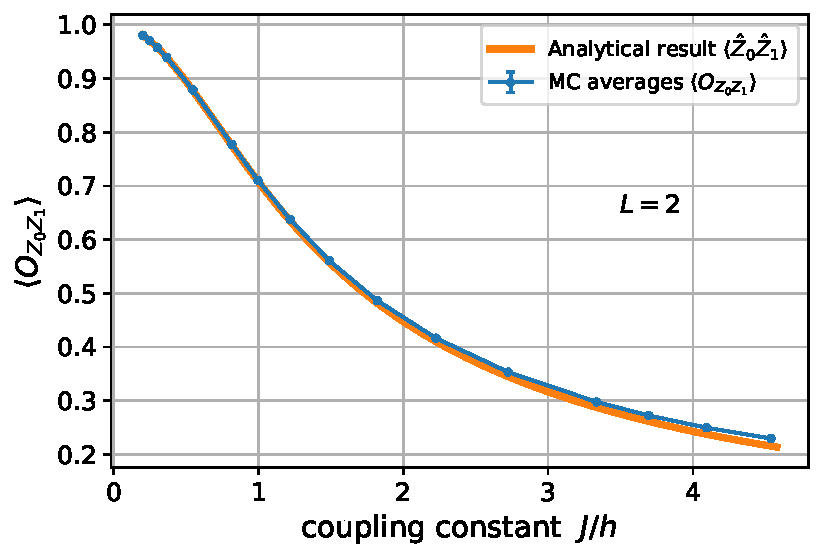
\includegraphics[width=\textwidth]{images/2_site/O_Z0Z1.pdf}
        \caption{Monte Carlo average $\expval{O_{Z_0 Z_1}}$ vs. $J/h$.}
        \label{expval_O_ZZ_vs_J/h_2}
    \end{subfigure}
    \caption{Comparing analytical results obtained by exactly diagonalizing the quantum Hamiltonian ($1d$)  with the numerical results obtained from performing Monte Carlo on the effective classical model $(1+1d)$.}
    \label{expval_O_vs_J/h_2}
\end{figure}
%%% FIG %%%
\FloatBarrier
As can be seen from Fig. \ref{expval_O_vs_J/h_2}, the Monte Carlo averages of the corresponding classical observables matches with the thermal expectation values of the quantum operators. At higher values of $J/h$, we can see some deviations arising due to the \textit{trotter error} despite the high MC acceptance rate.

Therefore, the modified Monte Carlo algorithm successfully  on the two site problem, and we will verify its relevance for higher spatial lattice sizes $N_x$ in the following section.

\section{Comparing Monte Carlo against exact diagonalization}
Analytical calculations for expectation values of quantum operators can only get us so far. The complexity of the calculation grows immensely on going from two sites to three sites. Therefore, it is not practical to rely on analytical calculations for evaluating quantum expectation values at higher lattice sizes $N_x>2$. Instead, we use the machinery of numerical exact diagonalization (ED) to numerically diagonalize the Hamiltonian for expectation value calculations. The quantum expectation value (at finite temperature) of an observable $\hat{\mathcal{O}}$ is calculated as follows, 
\begin{equation}
    \langle \hat{\mathcal{O}} \rangle =  \frac{1}{Z} \Tr(e^{-\beta \hat{H}} \hat{\mathcal{O}}) = \frac{\sum_{i} \mel{E_i}{\hat{\mathcal{O}}}{E_i} \: e^{-\beta E_i}}{\sum_i \braket{E_i}{E_i} e^{-\beta E_i}}
\end{equation}
where we calculate the trace over the energy eigenbasis. These quantum thermal expecatation values can then be compared with the Monte Carlo averages of the corresponding classical observables.

For verification purposes, we take the highest spatial lattice size possible for exact diagonalization calculations, i.e., $N_x = 13$ (due to exponentially increasing computational and memory costs). This is also an interesting lattice size to work with since standard Metropolis Monte Carlo breaks the subsystem symmetries at this lattice size leading to biased sampling. The introduction of alignment flips restores ergodicity in our classical model, and this benchmarking will serve as a test to whether our modified Monte Carlo algorithm captures the correct dynamics of the quantum system.

\subsection{Ground state simulations}
The ground state properties of the quantum system are probed by considering the $\beta h \to \infty$ limit. This is because it is the combination $\beta h$ (or $\beta J$) which enters the partition function,
\begin{equation}
    \exp\qty[-\beta \hat{H}] = \exp\qty[\beta h \qty(\sum_i Z_i Z_{i+1} + \frac{J}{h} \sum_i X_i)].
\end{equation}
Thus, for the purposes of our ground state simulations, we choose $\beta h= 2.50$ $(\beta = 50, \: h = 0.05)$. If we desire to simulate our model in the parameter range $J/h \in [a, b]$ and $\Delta \tau = 1$, then the range of $K$ chosen for MC simulations is such that
\begin{equation}
    K_i =-\frac{1}{2} \ln \tanh(h\cdot b), \qquad K_f =-\frac{1}{2} \ln \tanh(h\cdot a) 
\end{equation}   

\subsubsection{Monte Carlo setup}
\begin{itemize}[label={}]
    \setlength{\itemsep}{0.1em}
    \item \texttt{spatial lattice size $N_x = $ 13}
    \item \texttt{temporal lattice size $N_\tau = $ 50}
    \item \texttt{trotter unit $\Delta \tau = \texttt{1} $}
    \item \texttt{coupling parameter $Y = \texttt{0.05}$}
    \item \texttt{coupling parameter $K \in [\texttt{0.76}, \: \texttt{2.64}]$}
    \item \texttt{no of equilibration sweeps = \texttt{1.0e3}}
    \item \texttt{no of sampling sweeps $N_\text{samp} = $ 2$\tau \: \cdot$ 1.0e4}
    \item \texttt{sampling step size = 2$\tau $ }
\end{itemize}

\subsubsection{Exact diagonalization setup}
\begin{itemize}[label={}]
    \setlength{\itemsep}{0.1em}
    \item \texttt{spatial lattice size $N_x = $ 13}
    \item \texttt{interaction parameter $h = \texttt{0.05}$} 
    \item \texttt{field strength parameter $J \in [\texttt{0.005}, \:\texttt{0.22}]$} 
    \item \texttt{inverse temperature $\beta = \texttt{50}$}
\end{itemize}

%%% FIG %%%
\begin{figure}[!htb]
    \centering
    \begin{subfigure}[b]{0.55\textwidth}
        \centering
        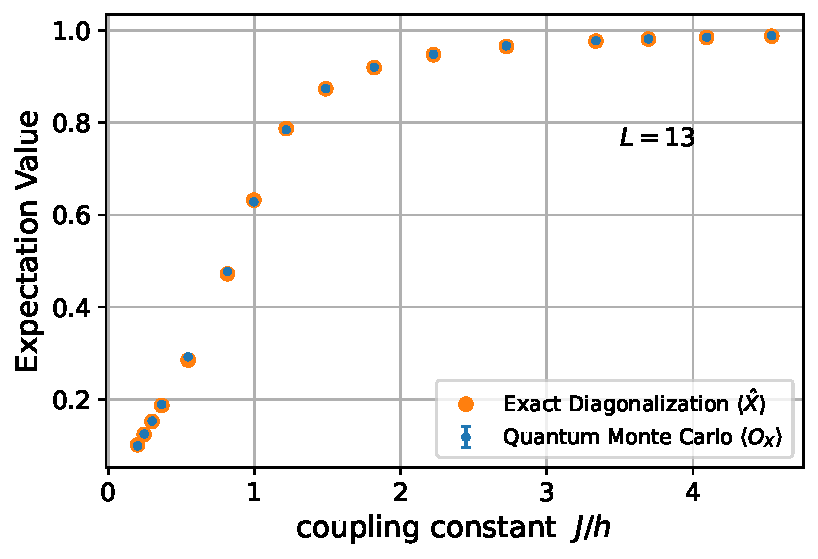
\includegraphics[width=\textwidth]{images/13_site/L=13_X.pdf}
    \end{subfigure}
    \caption{Comparing ED results for $\langle \hat{X} \rangle$ with MC average $\expval{O_X}$ at $\beta = 2.5$.}
    \label{expvalX_ED_vs_MC_13}
\end{figure}
%%% FIG %%%
\vspace*{1em}

%%% FIG %%%
\begin{figure}[!htb]
    \centering
    \begin{subfigure}[b]{0.5\textwidth}  %keep total sum <1 to show in same line
        \centering
        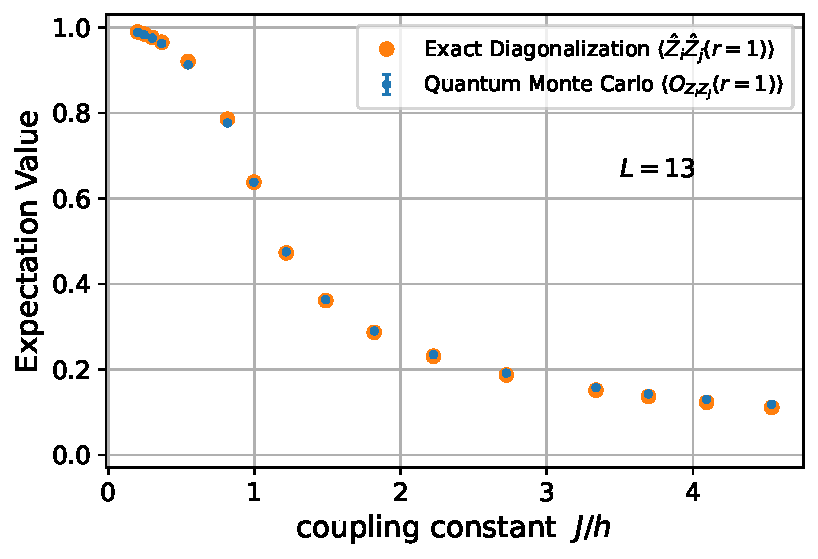
\includegraphics[width=\textwidth]{images/13_site/L=13_ZZ(r=1).pdf}
        \caption{$r \equiv |i-j| = 1$.}
    \end{subfigure}
\end{figure}
    \vspace*{1em}
\begin{figure}\ContinuedFloat
    \centering
    \begin{subfigure}[b]{0.5\textwidth}
        \centering
        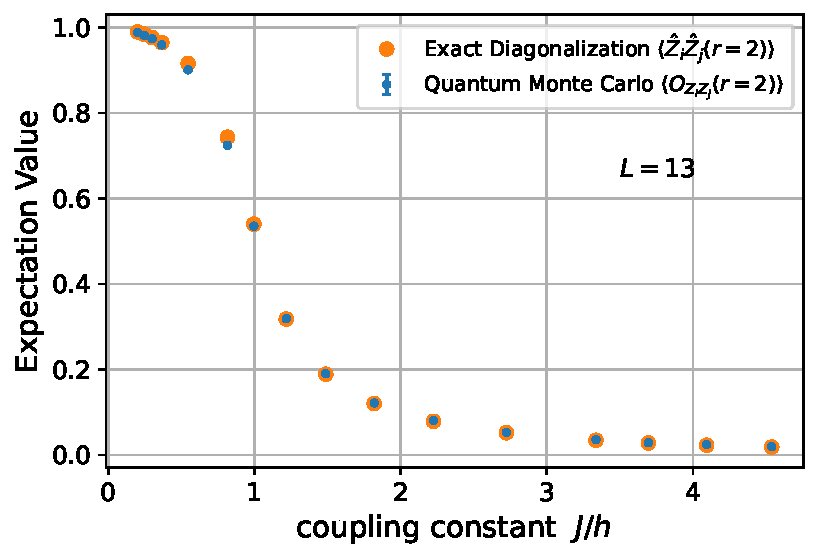
\includegraphics[width=\textwidth]{images/13_site/L=13_ZZ(r=2).pdf}
        \caption{$r \equiv |i-j| = 2$.}
    \end{subfigure}
    \begin{subfigure}[b]{0.49\textwidth}
        \centering
        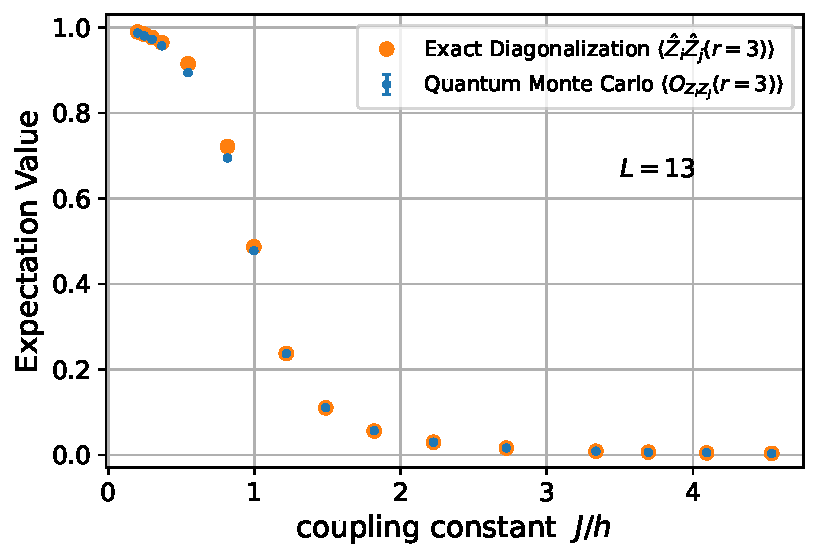
\includegraphics[width=\textwidth]{images/13_site/L=13_ZZ(r=3).pdf}
        \caption{$r \equiv |i-j| = 3$.}
    \end{subfigure}
    \caption{Comparing ED results for $\langle \hat{Z}_i \hat{Z}_j \rangle$ with MC average $\langle O_{Z_i Z_j} \rangle$ at $\beta = 2.5$.}
    \label{expvalZZ_ED_vs_MC_13}
\end{figure}
The benchmark plots in Figs.~\ref{expvalX_ED_vs_MC_13} and~\ref{expvalZZ_ED_vs_MC_13} clearly show that the Monte Carlo averages match very closely (within error bars) with the exact diagonalization expectation values, except for the slight variations in $Z_i Z_j$ expectation values as $|i-j|$ increases, which appear due to periodic boundary effects.

\subsection{Finite temperature simulations}
The machinery of our quantum Monte Carlo simulations can also be used to perform finite temperature simulations of our model. Since $\beta h = Y \cdot N_\tau$ acts like a temperature scale in our model, we can simulate finite temperature features by choosing $\beta h < 1$. 

\subsubsection{Monte Carlo setup}
Ideally, for a Monte Carlo simulation, having a large value of $N_\tau$ is necessary for reducing the trotter error and ensuring convergence to the correct results. Therefore, for the $ Y \cdot N_\tau < 1$ combination, $Y$ should be as small as possible while also ensuring that the order of magnitude stays roughly the same as $K$ (to prevent freezing of spins along the spatial axis). 

The only relevant parameters entering the Monte Carlo calculation are $Y, \:K, $ and $N_\tau$. We choose $Y = 0.05$, the same as before, and $N_\tau = 10$, implying that the value of the temperature scale is $\beta h = Y \cdot N_\tau = 0.5$. The values of $K$ are chosen accordingly to explore the region close to $J/h = 1$. 

The parameters are chosen as follows
\begin{itemize}[label={}]
    \setlength{\itemsep}{0.1em}
    \item \texttt{spatial lattice size $N_x = $ 13}
    \item \texttt{temporal lattice size $N_\tau = $ 10}
    \item \texttt{trotter unit $\Delta \tau = \texttt{1} $}
    \item \texttt{coupling parameter $Y = \texttt{0.05}$}
    \item \texttt{coupling parameter $K \in [\texttt{1.15}, \: \texttt{2.30}]$}
    \item \texttt{no of equilibration sweeps = \texttt{1.0e3}}
    \item \texttt{no of sampling sweeps $N_\text{samp} = $ 2$\tau \: \cdot$ 1.0e4}
    \item \texttt{sampling step size = 2$\tau $ }
\end{itemize}

\subsubsection{Exact diagonalization setup}
The exact diagonalization calculations doesn't suffer from a spin freezing or trotterization error problem like the Monte Carlo simulations. Moreover, the expectation value calculation for a fixed value of $J/h$ only depends on the value of $\beta h$. This implies that we have a family of parameter pair solutions $(\beta, h)$ which satisfy the constraint $\beta h = C$ where $C$ is our desired temperature scale for the simulation. This family of parameter pairs $(\beta, h = C/\beta)$ gives the same results for the expectation value calculations. 

Thus, exploiting this extra degree of freedom, we pretend to work at unit temperature $\beta = 1$ in exact diagonalization calculations. Consequently, $h$ and $J$ are chosen as follows
\begin{subequations}
    \begin{align}
        &h = \beta h = N_\tau \:Y \\
        &J = \beta J = N_\tau \: \text{arctanh}(e^{-2K})
    \end{align}
\end{subequations}
where $Y$ value and $K$ ranges are chosen to be the same as the Monte Carlo parameters. The parameters are chosen as follows
\begin{itemize}[label={}]
    \setlength{\itemsep}{0.1em}
    \item \texttt{spatial lattice size $N_x = $ 13}
    \item \texttt{interaction parameter $h = N_\tau \:Y = \texttt{0.05}$} 
    \item \texttt{field strength parameter $J = N_\tau \: \textrm{arctanh}(e^{-2K}) \in [\texttt{0.01}, \:\texttt{0.1}]$} 
    \item \texttt{inverse temperature $\beta = \texttt{1}$}
\end{itemize}
%%% FIG %%%
\begin{figure}[!htb]
    \centering
    \begin{subfigure}[b]{0.55\textwidth}
        \centering
        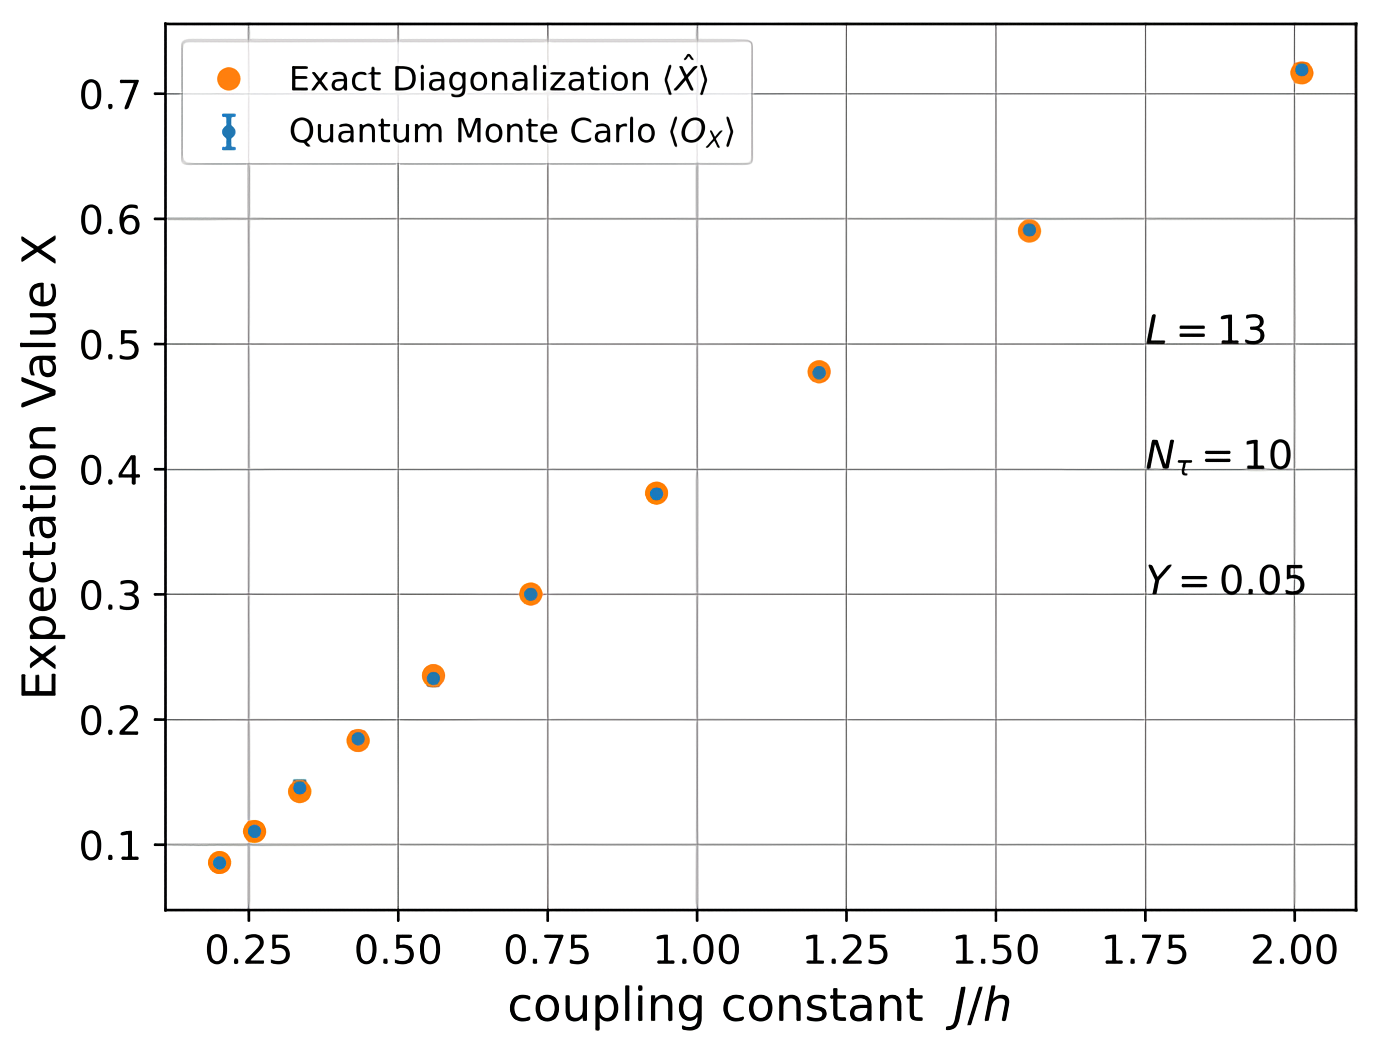
\includegraphics[width=\textwidth]{images/finite temps L13/X.png}
    \end{subfigure}
    \caption{Comparing ED results for $\langle \hat{X} \rangle$ with MC average $\expval{O_X}$ at $\beta = 0.5$.}
    \label{expvalX_ED_vs_MC_13_FT}
\end{figure}
%%% FIG %%%
\vspace*{1em}

%%% FIG %%%
\begin{figure}[!htb]
    \centering
    \begin{subfigure}[b]{0.49\textwidth}  %keep total sum <1 to show in same line
        \centering
        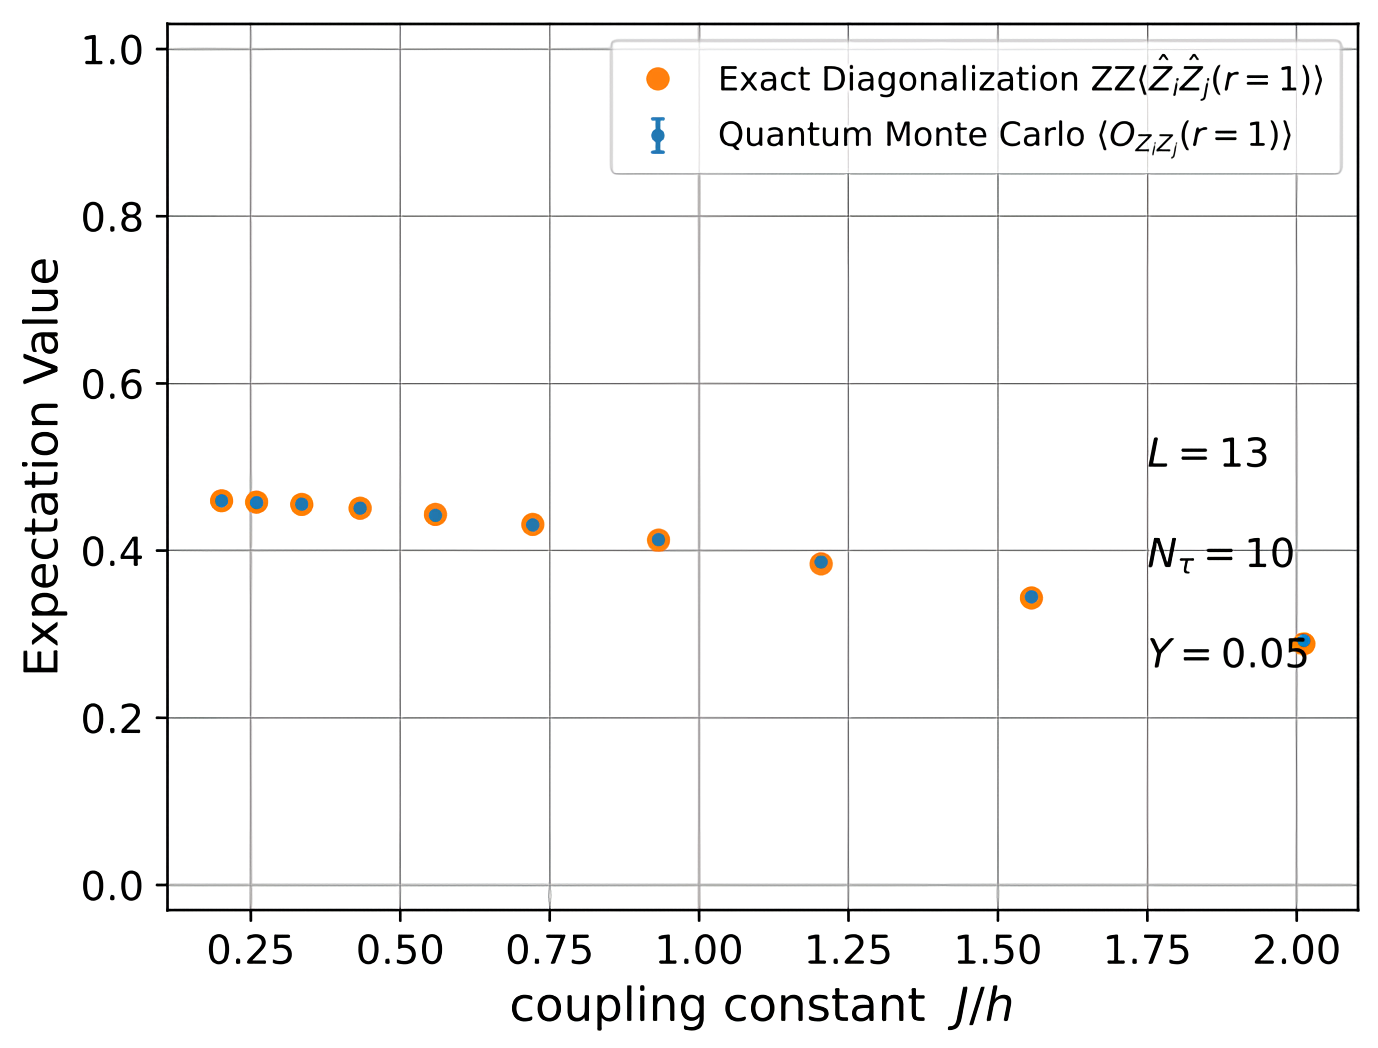
\includegraphics[width=\textwidth]{images/finite temps L13/ZZ1.png}
        \caption{$r \equiv |i-j| = 1$.}
    \end{subfigure}
    \begin{subfigure}[b]{0.49\textwidth}
        \centering
        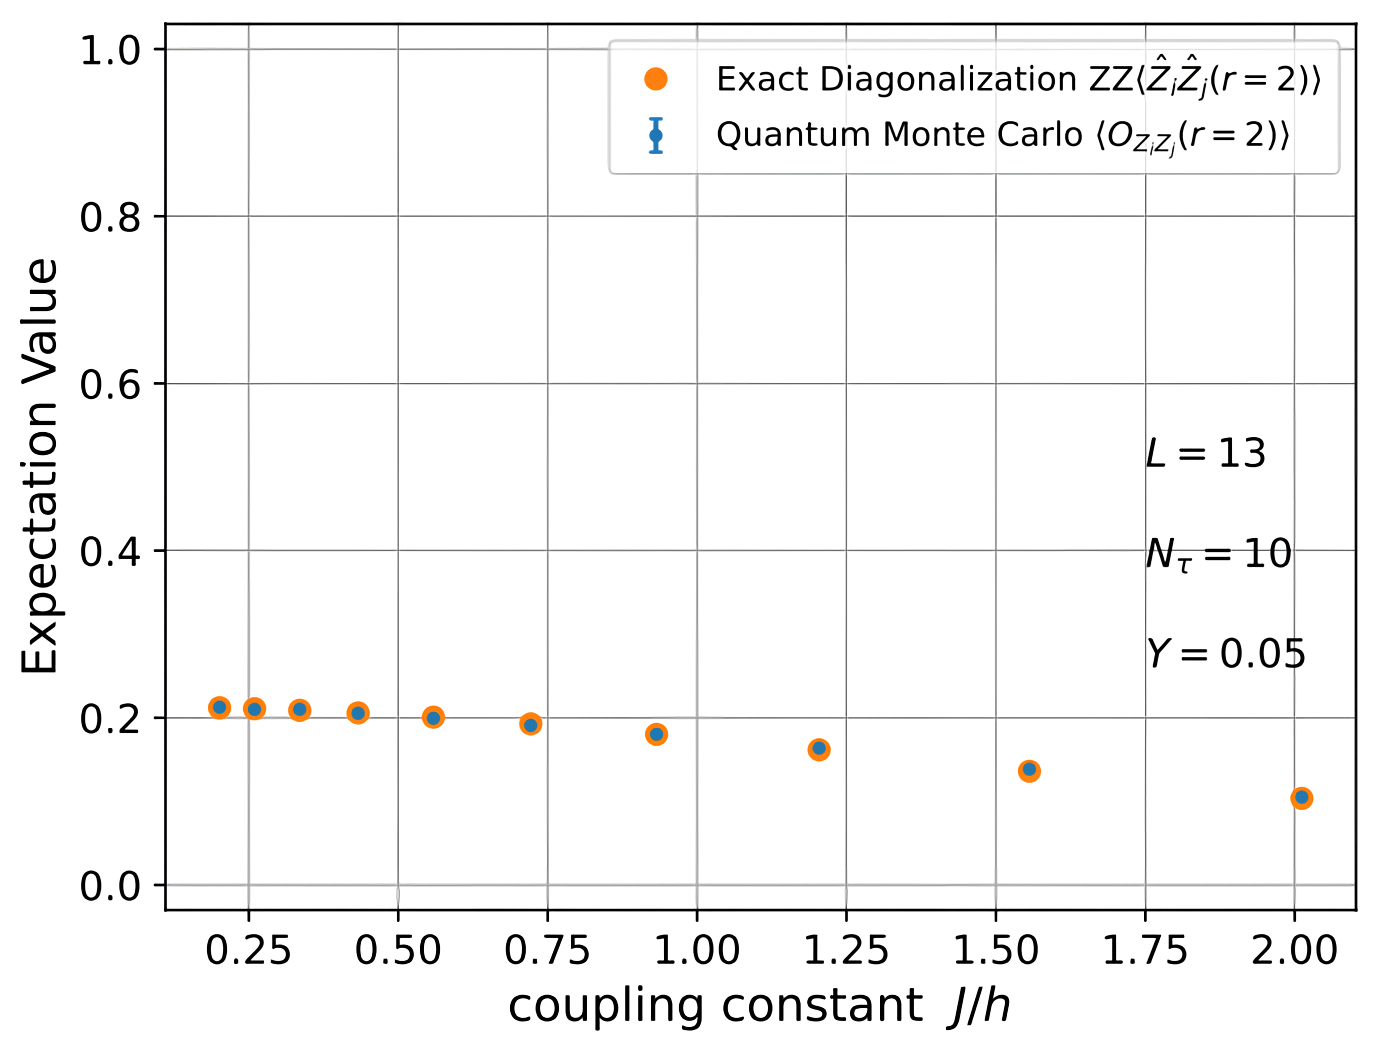
\includegraphics[width=\textwidth]{images/finite temps L13/ZZ2.png}
        \caption{$r \equiv |i-j| = 2$.}
    \end{subfigure}
    \caption{Comparing ED results for $\langle \hat{Z}_i \hat{Z}_j \rangle$ with MC average $\langle O_{Z_i Z_j} \rangle$ at $\beta = 0.5$.}
    \label{expvalZZ_ED_vs_MC_13_FT}
\end{figure}
\FloatBarrier
Figs.~\ref{expvalX_ED_vs_MC_13_FT} and~\ref{expvalZZ_ED_vs_MC_13_FT} again show very close matching of Monte Carlo averages with the exact diagonalization calculations, even at finite temperatures $\beta h < 1$. 

Thus, the ergodicity analysis and the benchmarking against exact digaonlization clearly suggest that our modified Metropolis Monte Carlo simulations are successful in simulating the model of interest. Therefore, we conclude that the proposed Metropolis algorithm is an effective numerical tool for understanding the phase structure of $\mathbb{Z}_2$ lattice gauge theory.

\section{Quantum phase transition}
The study of expectation values of operators in the previous sections highlighted variation in the value of the quantities at $T = 0$ as the coupling parameter $J/h$ is varied across a range. The variation of these quantities from a zero to a non-zero value is illustrates a change in phase. Since such a phase transition isn't driven by any thermal effects and is purely an artefact of the quantum fluctuations tuned by a variation in the nonthermal parameters, it is called a \textit{quantum phase transition}.

However, as noted in Chapter~\ref{chap:1}, it is impossible in theory for a system of finite size to undergo a phase transition. In simulations, the system sizes are often small in comparison to experiments, and understanding of finite size effects is important. An important tool for studying phase transitions in finite size systems is the Binder cumulant, and we recall
\begin{equation}
    U_L = 1 - \frac{\expval{\hat{m}^4}_L}{3\expval{\hat{m}^2}^2_L}
\end{equation}
where $|m|$ is like an order parameter characterizing the transition. But $Z_i$ is not a singlet compatible operator in the singlet Hilbert space $\mathcal{H}_s$
\begin{equation}
    \hat{F} \: Z_i \: \hat{F} = - Z_i
\end{equation}
Consequently, the magnetization operator
\begin{equation}
    \hat{m} = \frac{1}{N_x} \sum_{i=0}^{N_x-1} Z_i
\end{equation}
is also ill-defined. Therefore, magnetization isn't a valid operator in this subspace, let alone be an order parameter. However, even powers of magnetization, i.e., $\langle m^{2n} \rangle$ (for $n \in \mathbb{Z}^+$) are singlet compatible and the definition of the Binder cumulant is still valid.

\subsection{Classical analog of the Binder cumulant}
Let us consider the elementary operator $\hat{m}^{2n}$ which is used to construct the Binder cumulant. The classical analog of the $\hat{m}^{2n}$ operator is calculated by substituting $\hat{\mathcal{O}} =  \hat{Z}_i \hat{Z}_j$ in Eq.~\eqref{generalop}.
\begingroup
\allowdisplaybreaks
\begin{align}
    \cdot \langle {\hat{Z}_i \hat{Z}_j} \rangle &= \frac{1}{\mathcal{Z} }\qty(\prod_{l=0}^{N_\tau - 1} \sum_{\{\sigma_l \}, \mu_l, \lambda_l}) \frac{1}{N_\tau} \sum_{l_0 = 0}^{N_\tau - 1} \Bigg[\langle\{\mu_{l_0+1} \sigma _{l_0+1}\}|{e^{-\Delta \tau \hat{H}}{\hat{m}^{2n}}}|{\{\lambda_{l_0} \sigma _{l_0}\}} \rangle \qquad \qquad \nonumber\\
    &\qquad \qquad \qquad \qquad \qquad \qquad \qquad \qquad \prod_{l \neq l_0} \mel{\{\mu_{l+1} \sigma _{l+1}\}}{e^{-\Delta \tau \hat{H}}}{\{\lambda_{l} \sigma _{l}\}} \Bigg] \nonumber \\
    & =  \frac{1}{\mathcal{Z} }\qty(\prod_{l=0}^{N_\tau - 1} \sum_{\{\sigma_l \}, \mu_l, \lambda_l}) \frac{1}{N_\tau} \sum_{l_0 = 0}^{N_\tau - 1} \Bigg[\mel{\{\mu_{l_0+1} \sigma _{l_0+1}\}}{e^{-\Delta \tau \hat{H}}}{\{\lambda_{l_0} \sigma _{l_0}\}} (\lambda_{l_0} \sigma^i_{l_0})(\lambda_{l_0} \sigma^j_{l_0}) \qquad \qquad \nonumber \\ 
    & \qquad \qquad \qquad \qquad \qquad \qquad \qquad \qquad \prod_{l \neq l_0} \mel{\{\mu_{l+1} \sigma _{l+1}\}}{e^{-\Delta \tau \hat{H}}}{\{\lambda_{l} \sigma _{l}\}}\Bigg] \nonumber \\ 
    & = \frac{1}{\mathcal{Z} }\qty(\prod_{l=0}^{N_\tau - 1} \sum_{\{\sigma_l \}, \mu_l, \lambda_l}) \qty[\frac{1}{N_\tau} \sum_{l_0 = 0}^{N_\tau - 1}  \qty(\frac{1}{N_x} \sum_{i=0}^{N_x-1} \sigma^i_{l_0})^{2n}]  \nonumber  \\
    & \qquad \qquad \qquad \qquad \qquad \qquad \qquad \qquad\qty[\prod_{l = 0}^{N_\tau - 1} \mel{\{\mu_{l+1} \sigma _{l+1}\}}{e^{-\Delta \tau \hat{H}}}{\{\lambda_{l} \sigma _{l}\}}]
\end{align}
\endgroup

\end{document}